\documentclass[11pt]{article}
\usepackage[utf8]{inputenc}	% Para caracteres en español
\usepackage{amsmath,amsthm,amsfonts,amssymb,amscd}
\usepackage{multirow,booktabs}
\usepackage[table]{xcolor}
\usepackage{fullpage}
\usepackage{lastpage}
\usepackage{enumitem}
\usepackage{fancyhdr}
\usepackage{mathrsfs}
\usepackage{wrapfig}
\usepackage{setspace}
\usepackage{calc}
\usepackage{multicol}
\usepackage{cancel}
\usepackage[retainorgcmds]{IEEEtrantools}
\usepackage[margin=1cm]{geometry}
\usepackage{amsmath}
\newlength{\tabcont}
\setlength{\parindent}{0.0in}
\setlength{\parskip}{0.05in}
\usepackage{empheq}
\usepackage{framed}
\usepackage[most]{tcolorbox}
\usepackage{xcolor}
\usepackage{graphicx}
\usepackage{listings}
% -- Basic formatting
\usepackage[utf8]{inputenc}
\usepackage[english]{babel}
\usepackage{times}
\usepackage{caption}
\usepackage{subcaption}
\usepackage{placeins}
\setlength{\parindent}{0pt}
\usepackage{indentfirst}% -- Defining colors:
\usepackage[dvipsnames]{xcolor}
\definecolor{codegreen}{rgb}{0,0.6,0}
\definecolor{codegray}{rgb}{0.5,0.5,0.5}
\definecolor{codepurple}{rgb}{0.58,0,0.82}
\definecolor{backcolour}{rgb}{0.95,0.95,0.92}% Definig a custom style:
\lstdefinestyle{mystyle}{
    backgroundcolor=\color{backcolour},   
    commentstyle=\color{codepurple},
    keywordstyle=\color{NavyBlue},
    numberstyle=\tiny\color{codegray},
    stringstyle=\color{codepurple},
    basicstyle=\ttfamily\footnotesize\bfseries,
    breakatwhitespace=false,         
    breaklines=true,                 
    captionpos=t,                    
    keepspaces=true,                 
    numbers=left,                    
    numbersep=5pt,                  
    showspaces=false,                
    showstringspaces=false,
    showtabs=false,                  
    tabsize=2
}% -- Setting up the custom style:
\lstset{style=mystyle}
\lstset{
  style=mystyle,
  framexleftmargin=3.5mm,
  rulesepcolor=\color{black},
  linewidth=0.6\linewidth,
  xleftmargin=12pt,
  aboveskip=12pt,
  belowskip=12pt
}
\colorlet{shadecolor}{orange!15}
\parindent 0in
\parskip 1pt
\geometry{margin=1in, headsep=0.25in}
\theoremstyle{definition}
\newtheorem{defn}{Definition}
\newtheorem{reg}{Rule}
\newtheorem{exer}{Exercise}
\newtheorem{note}{Note}
\graphicspath{ {./images/} }
\begin{document}
\setcounter{section}{0}
\title{MIE223 Lecture Notes}

\thispagestyle{empty}

\begin{center}
{\LARGE \bf Centrality,
Connected Components,
and Communities}\\
{\large MIE223}\\
Winter 2025
\end{center}
\section{Centrality,
Connected Components,
and Communities}

\begin{note}
centrality can be determined by degree
\end{note}

\subsection{what does degree not capture}

cut vertices connect two components but does not have a high degree

\subsection{shortest path in a network}
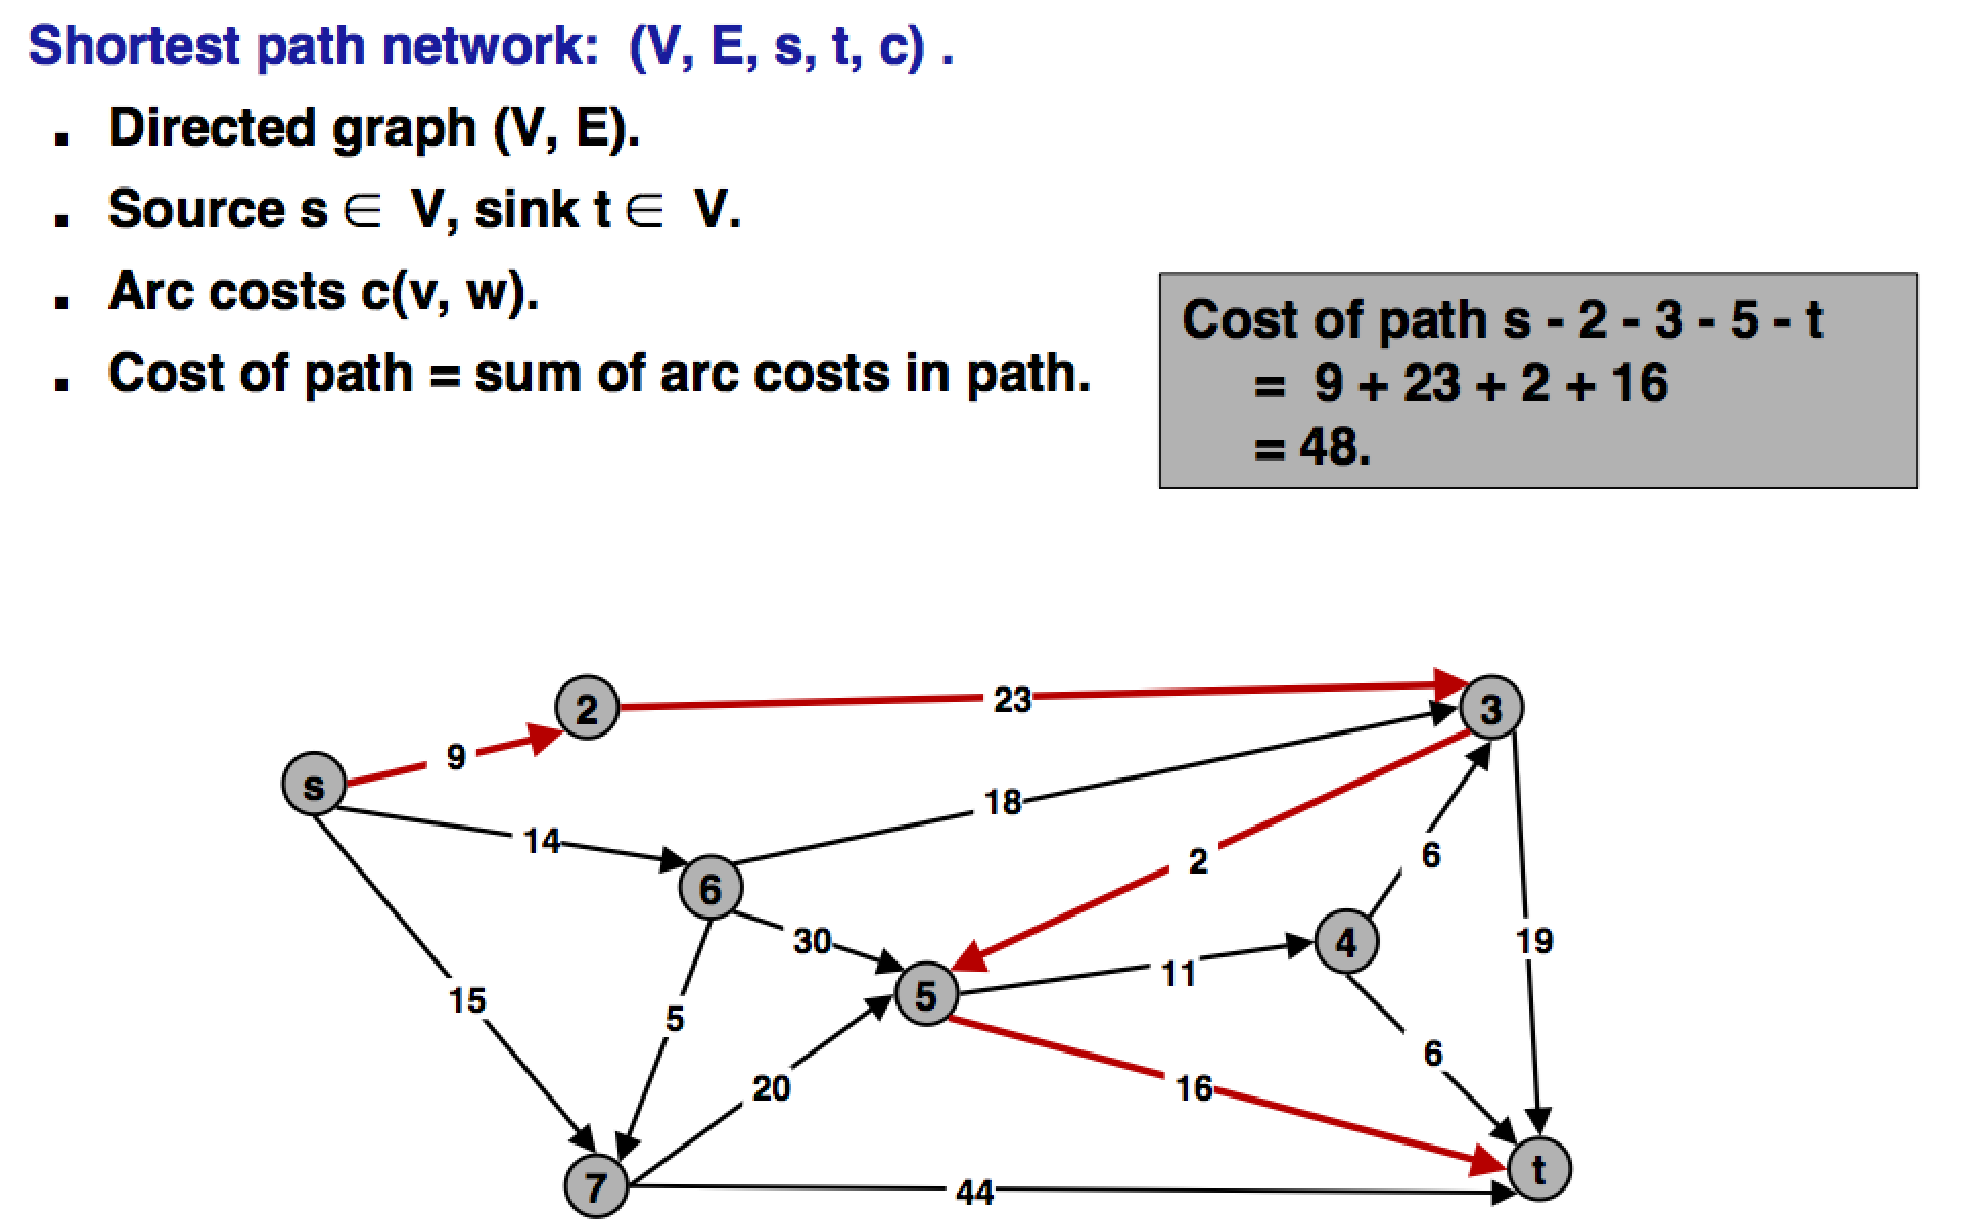
\includegraphics[width=\textwidth/2]{16.png}

\subsection{Betweenness: centrality capturing brokerage}
Intuition: how many pairs of individuals
would have to go through you in order to
reach one another in the minimum number
of hops?

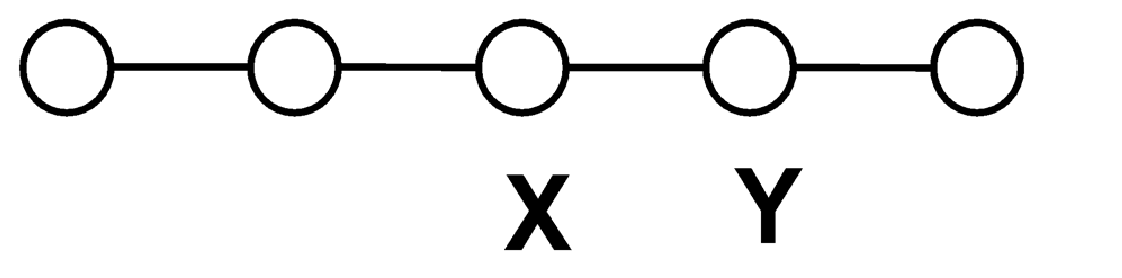
\includegraphics[width=\textwidth/2]{17.png}

\subsection{Betweenness: definition}
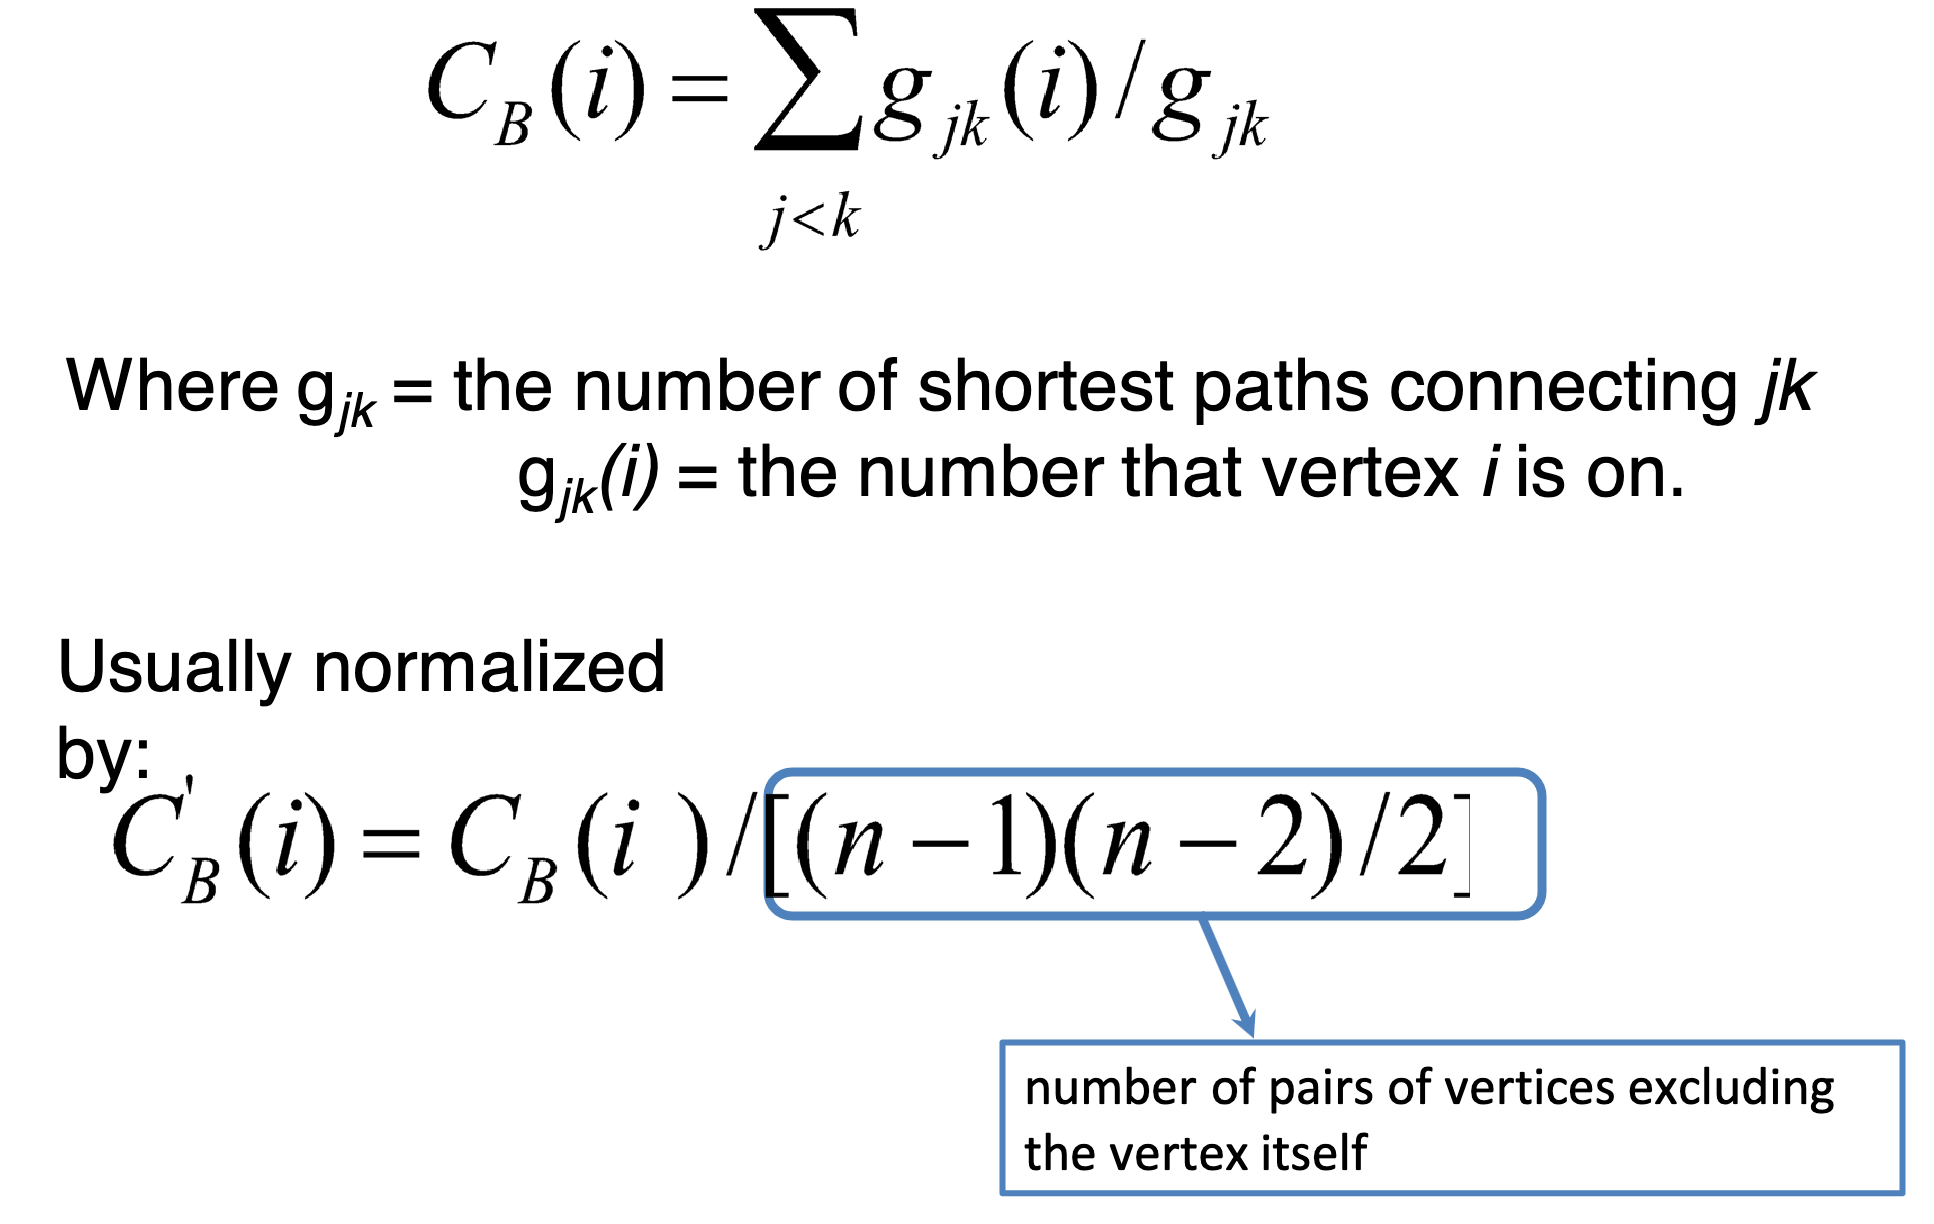
\includegraphics[width=\textwidth/2]{18.png}

a betweeness centrality for node i is the number of nodes
other than i who have to through i to interact with each other

g$_{jk}$(i) is a subset of g$_{jk}$

3 ordered pairs with 3 nodes equates to 9 paths

\subsection{quiz questions}
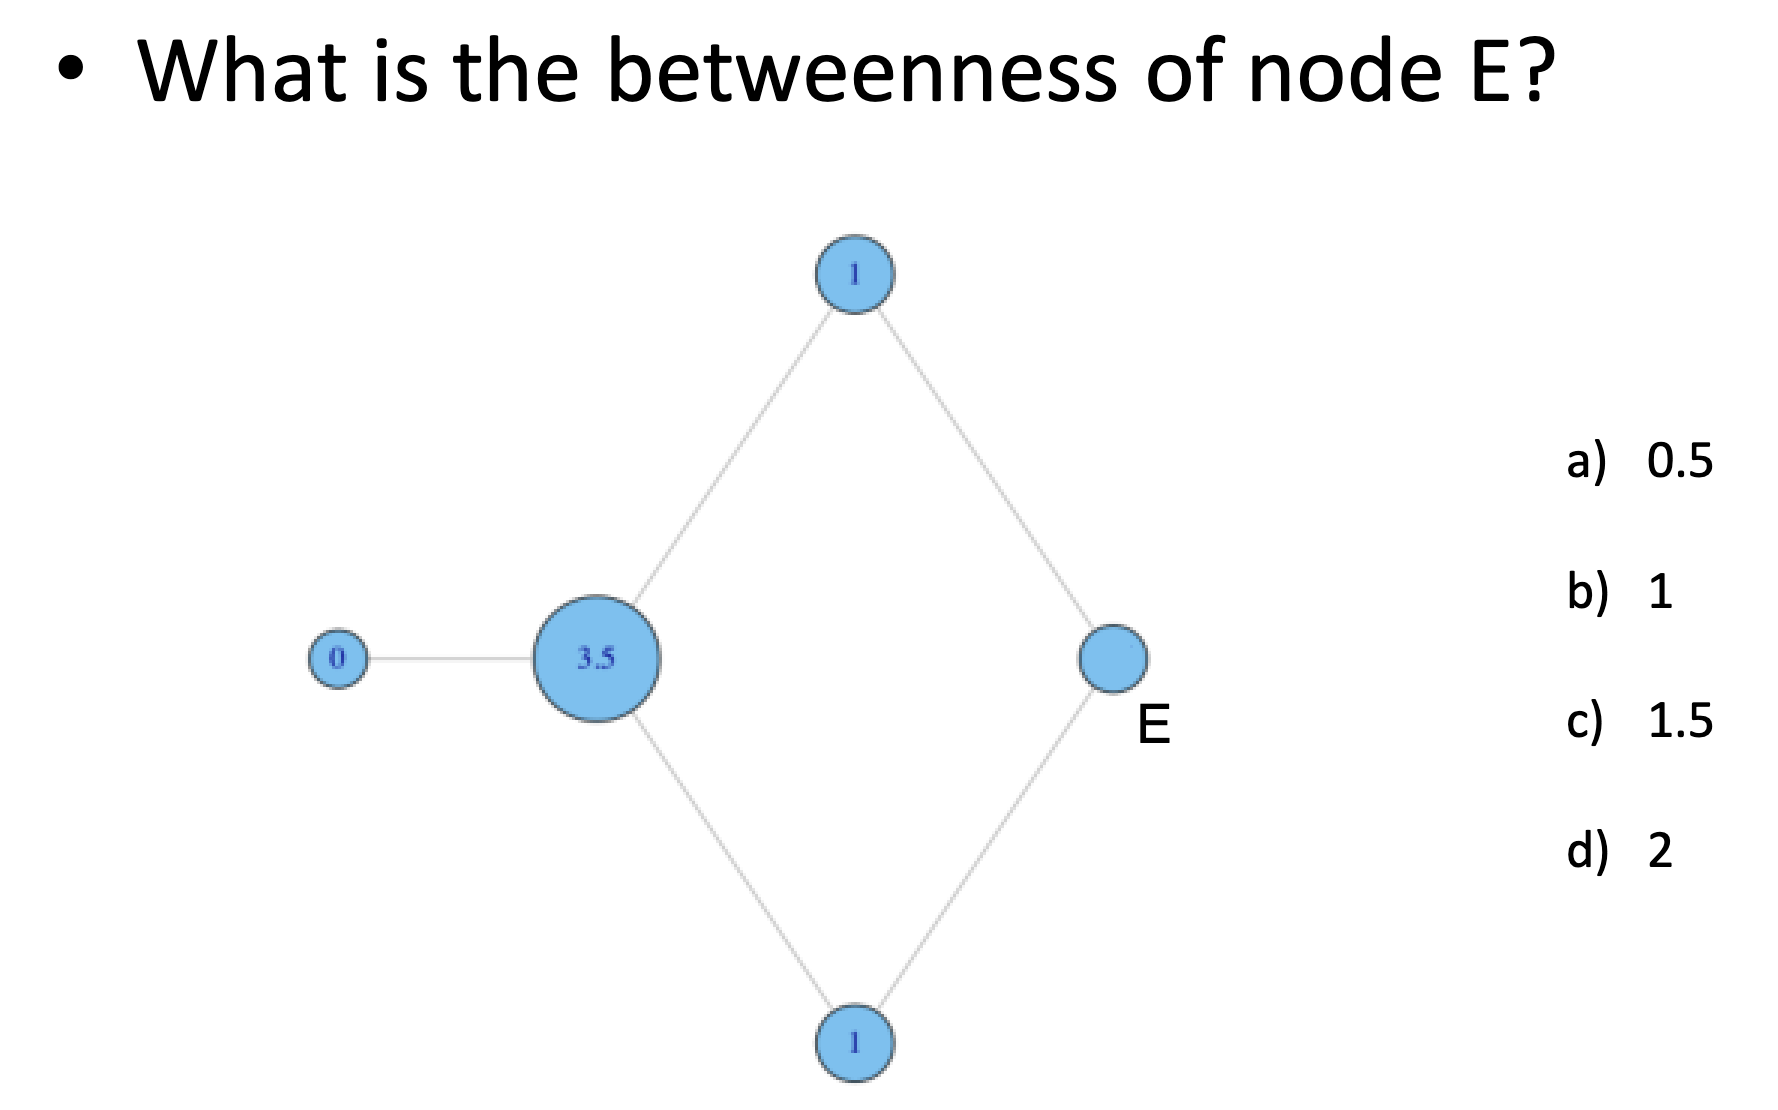
\includegraphics[width=\textwidth/2]{21.png}


what is betweenness of node E? a) 0.5
to get from 1 to 1 you can go through 3.5 or E

q2: G high betweenness low degree, A opposite
\section{Community detection}

Can we discover community
structure in an automated way?

\subsection{Connected components}
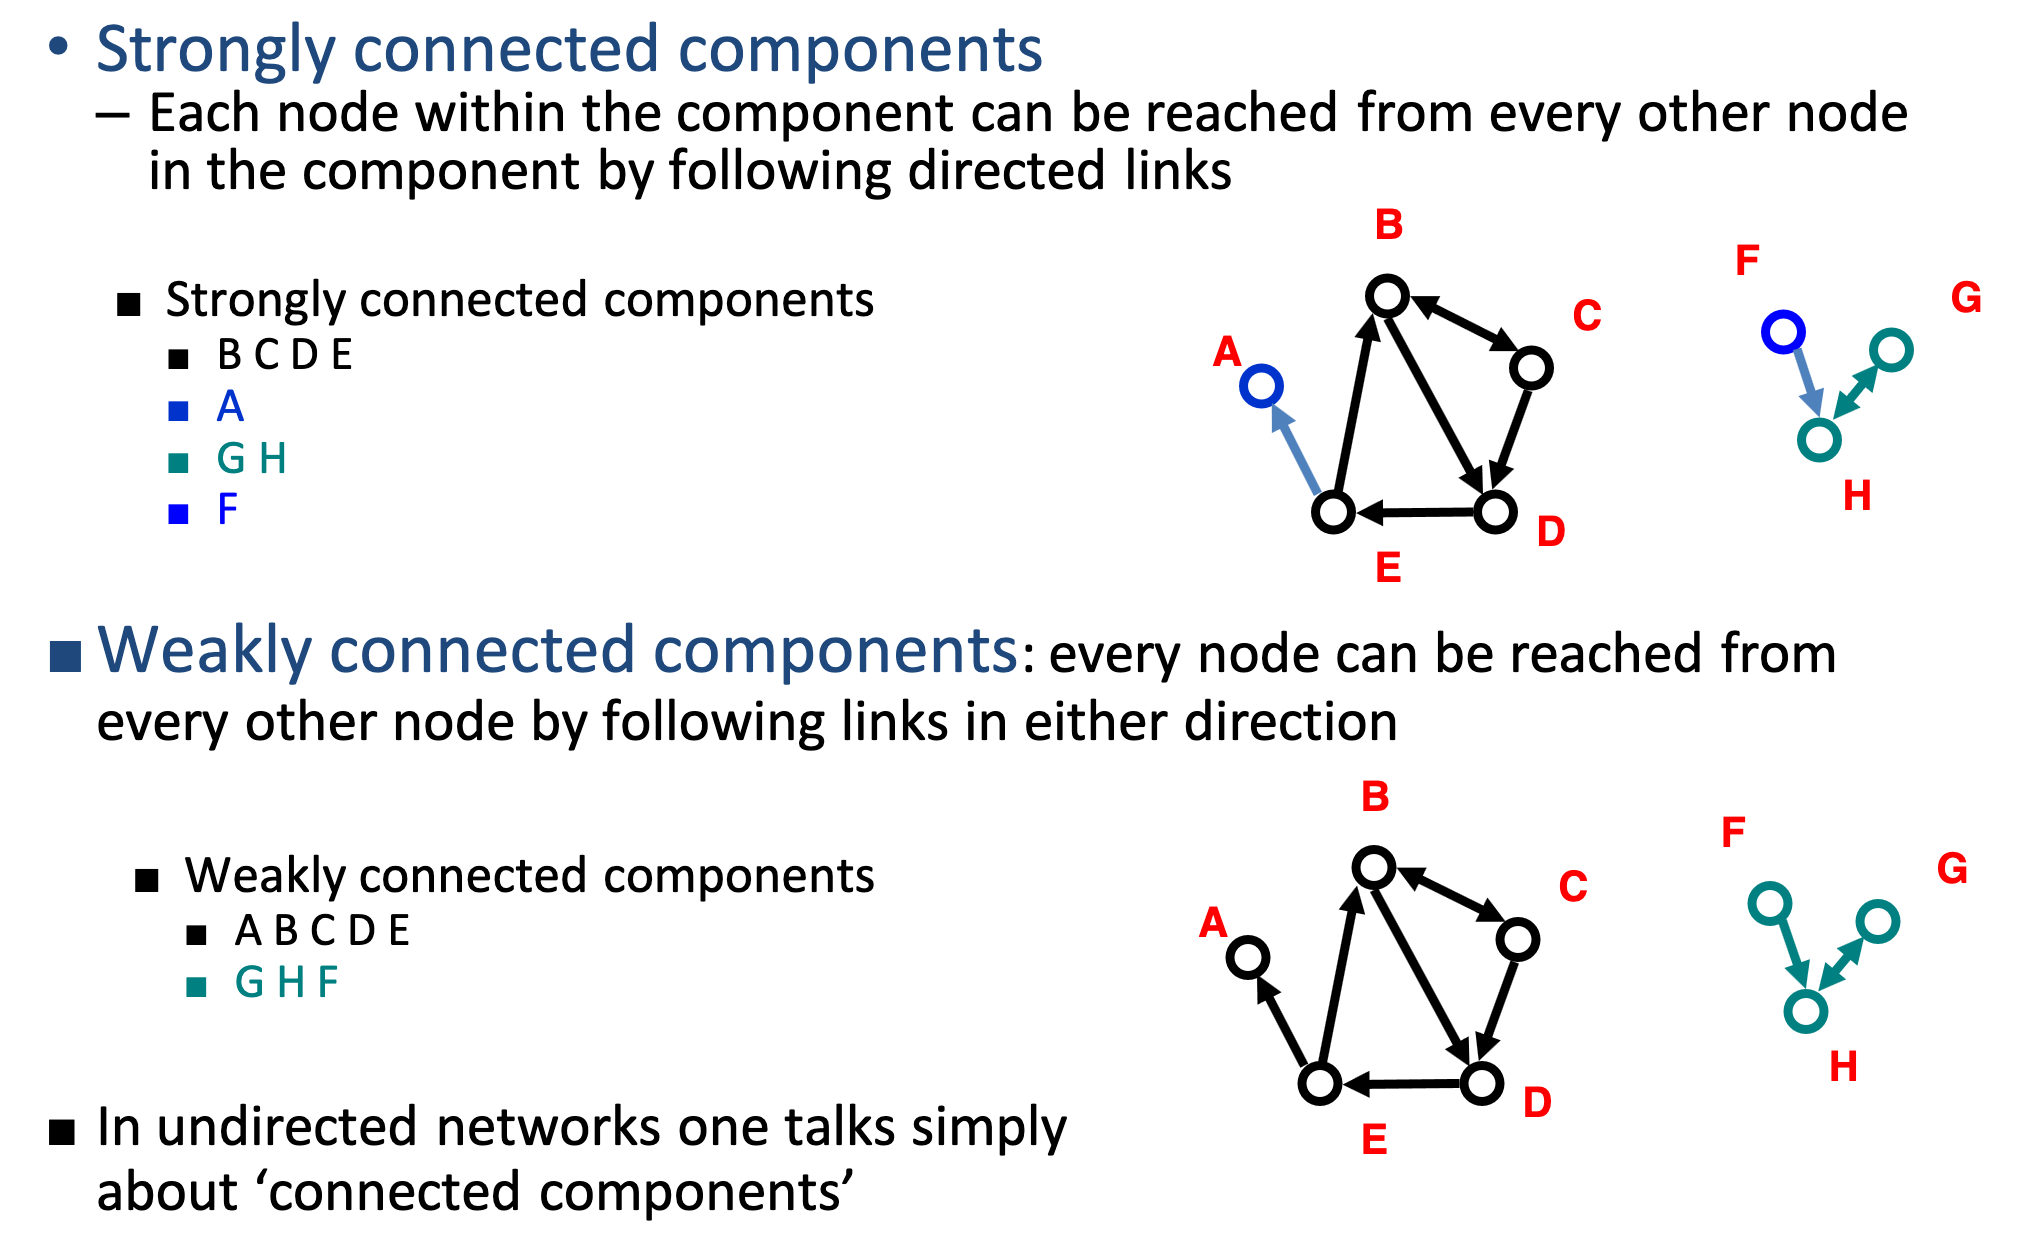
\includegraphics[width=\textwidth/2]{19.png}

\subsection{Giant component}
\begin{note}
    if the largest component encompasses a significant fraction of the
graph, it is called the giant component
\end{note}
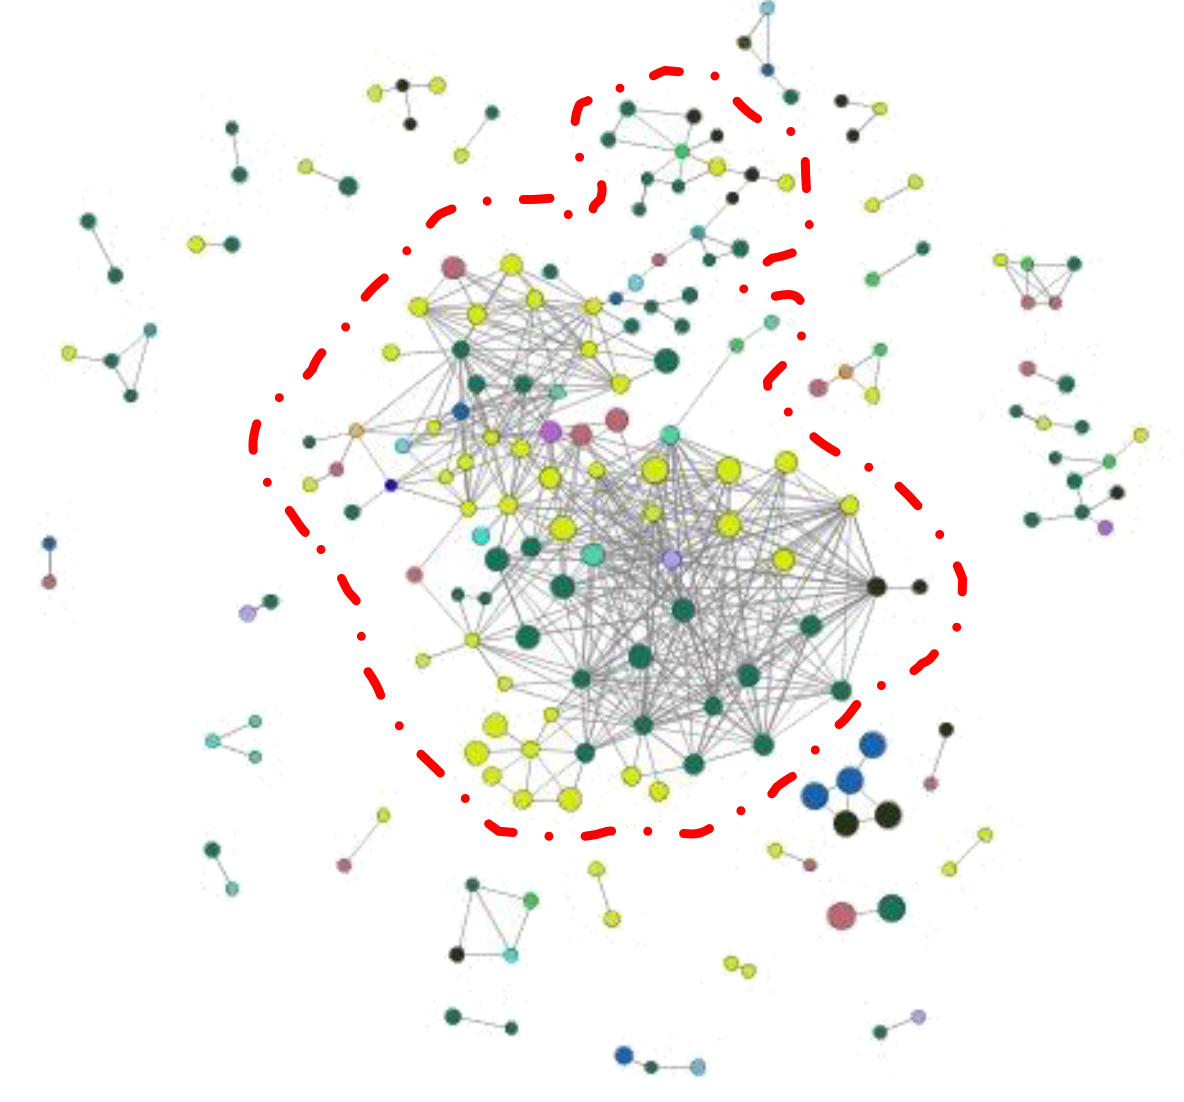
\includegraphics[width=\textwidth/4]{20.png}

great exam question: generalize equation for betweeness for edges
How many paths pass through this edge rather than the node
generalize the equation to directed graphs

\subsection{No 2 giant SCCs}
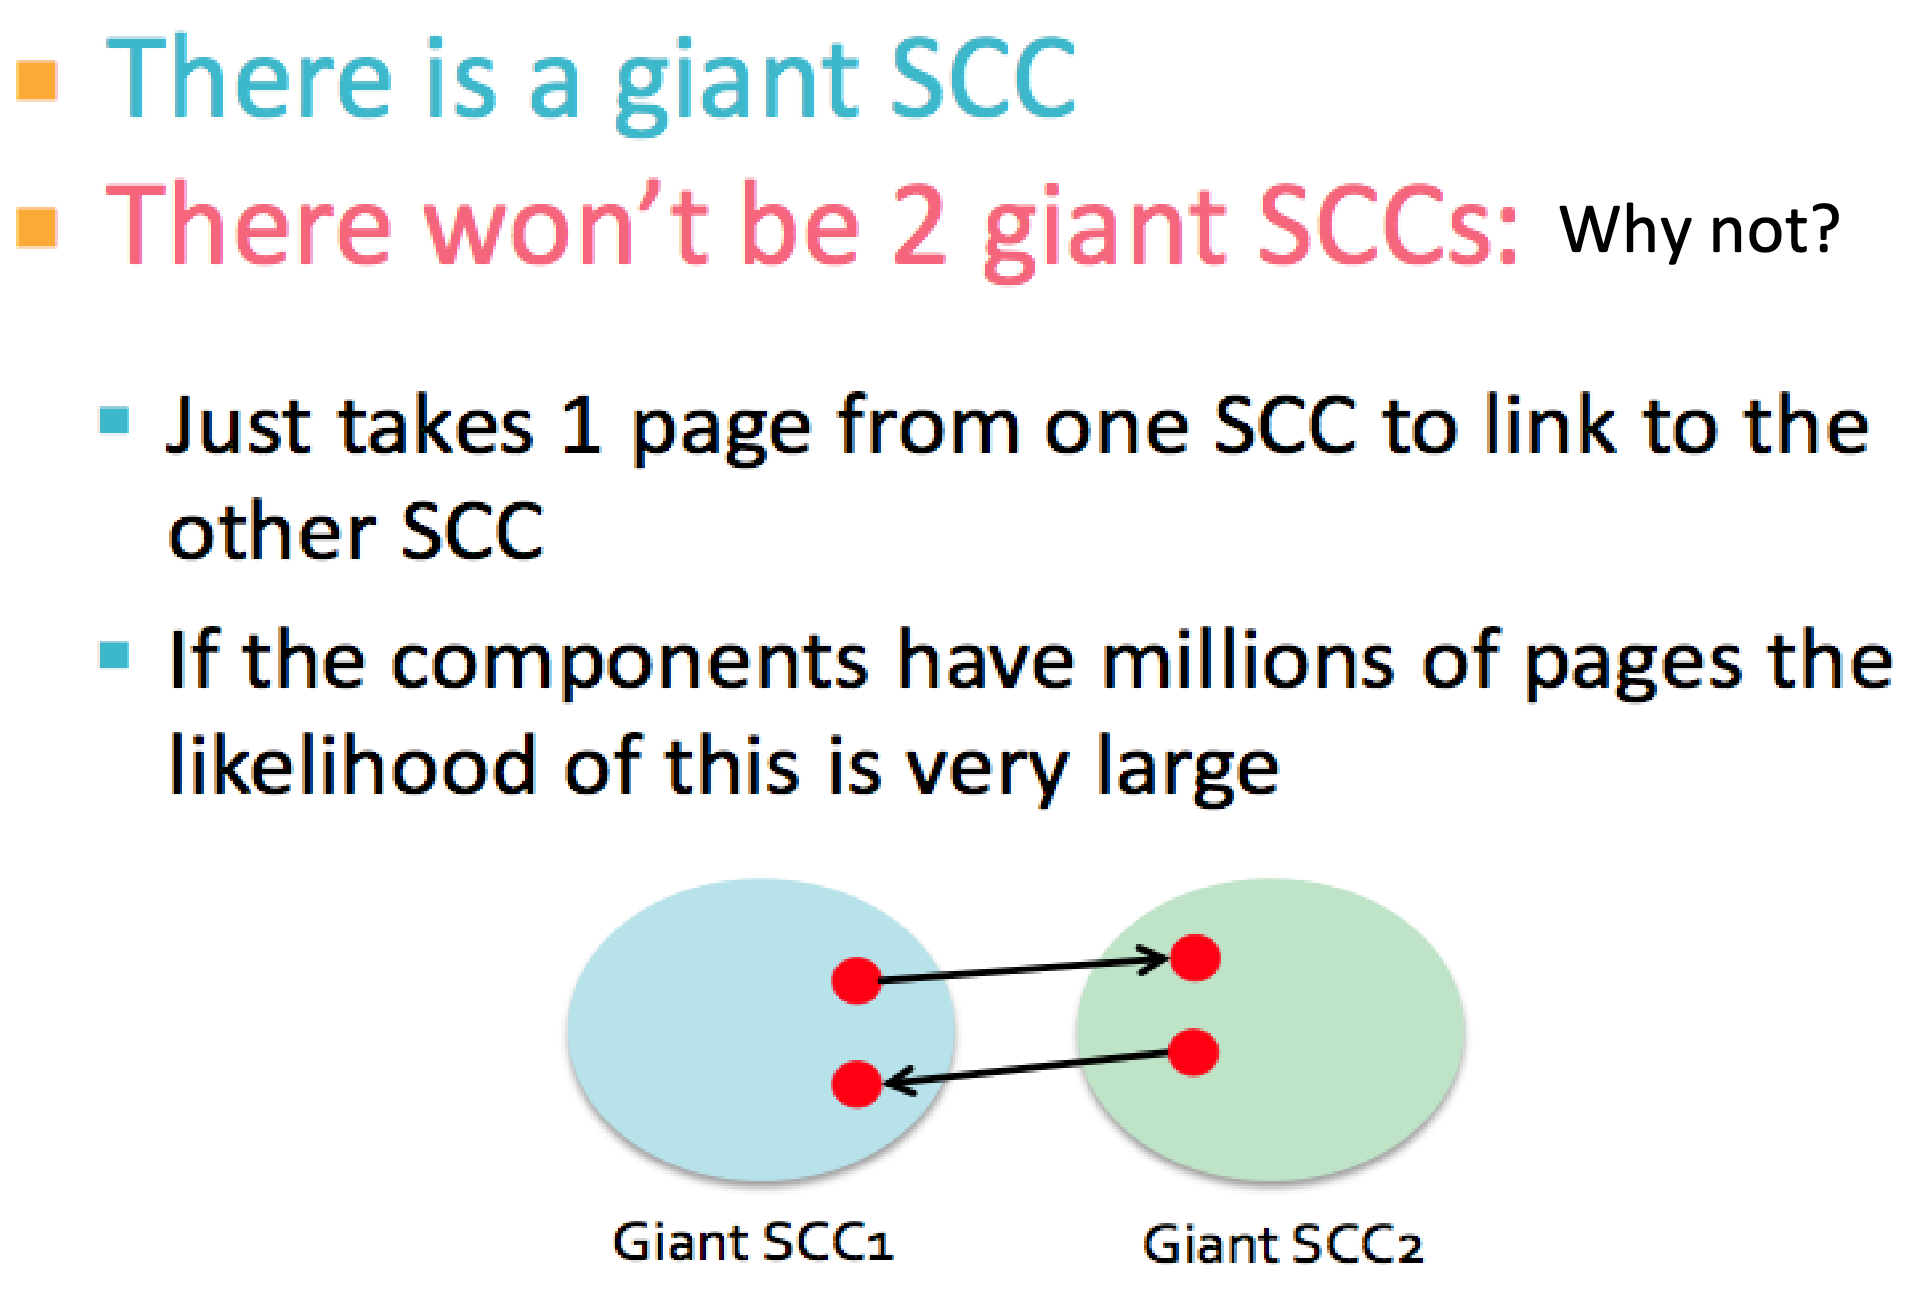
\includegraphics[width=\textwidth/4]{28.png}


\subsection{Splitting Zachary Karate Club}
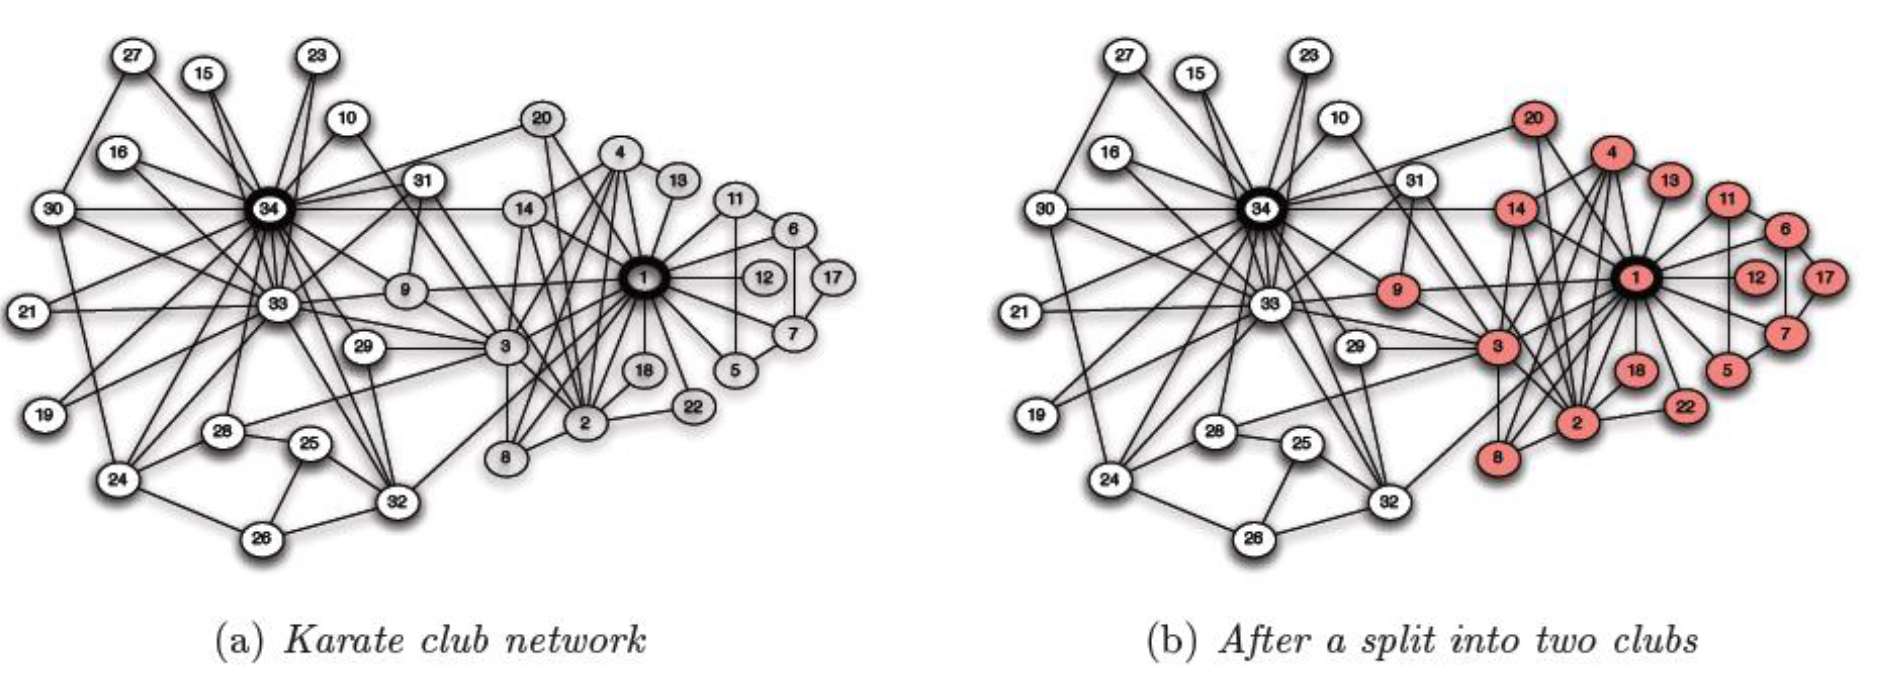
\includegraphics[width=\textwidth/2]{22.png}

do until (2 disconnected graphs)
compute betweennesses first for the given graph
remove edge has highest betweenness

\subsection{betweenness clustering}
Algorithm

\begin{itemize}
    \item Compute betweenness for all edges
    \item while (betweenness of any edge > threshold):
    \item remove edge with highest betweenness
    \item recalculate betweenness
\end{itemize}

Betweenness needs to be recalculated at each step

\begin{itemize}
    \item removal of an edge can impact the betweenness of another
    edge
    \item very expensive: all pairs shortest path – O(N$^3$)
    \item may need to repeat up to N times
    \item does not scale to more than a few hundred nodes, even with
    the fastest algorithms
\end{itemize}

\subsection{betweenness clustering:}
successively remove edges of highest betweenness (the bridges, or local
bridges), breaking up the network into separate components

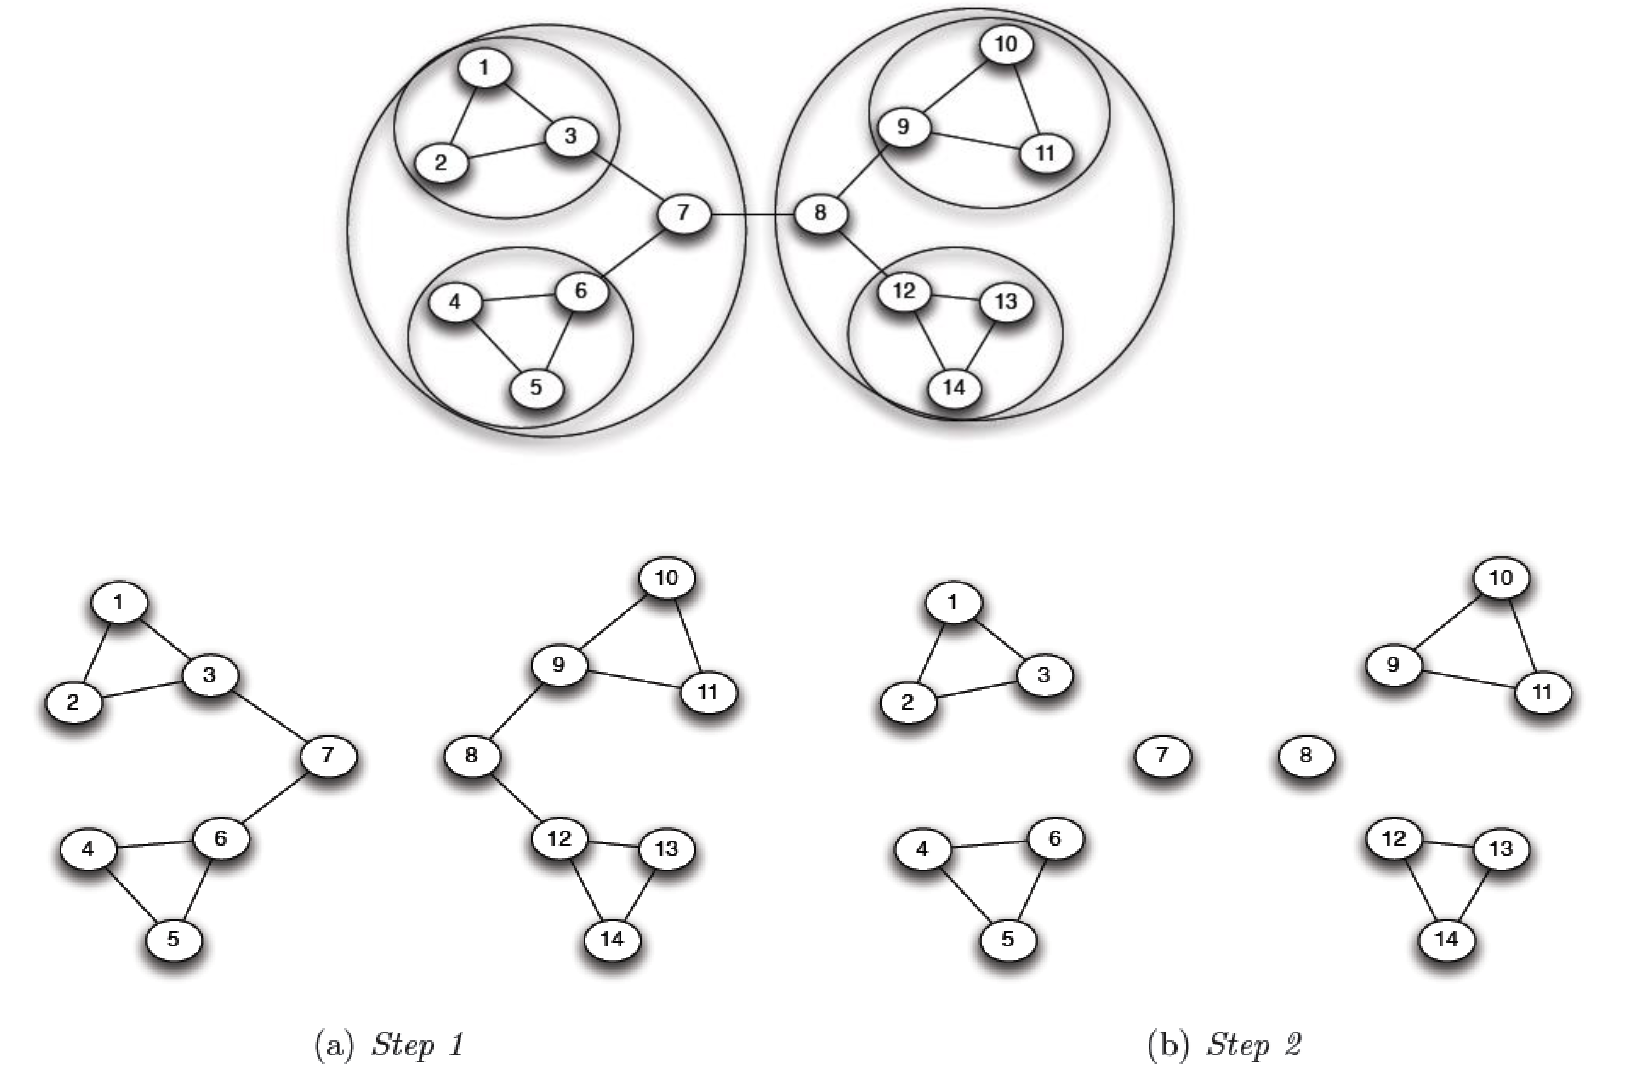
\includegraphics[width=\textwidth/2]{23.png}

\subsection{betweenness clustering algorithm \& the karate club data set}
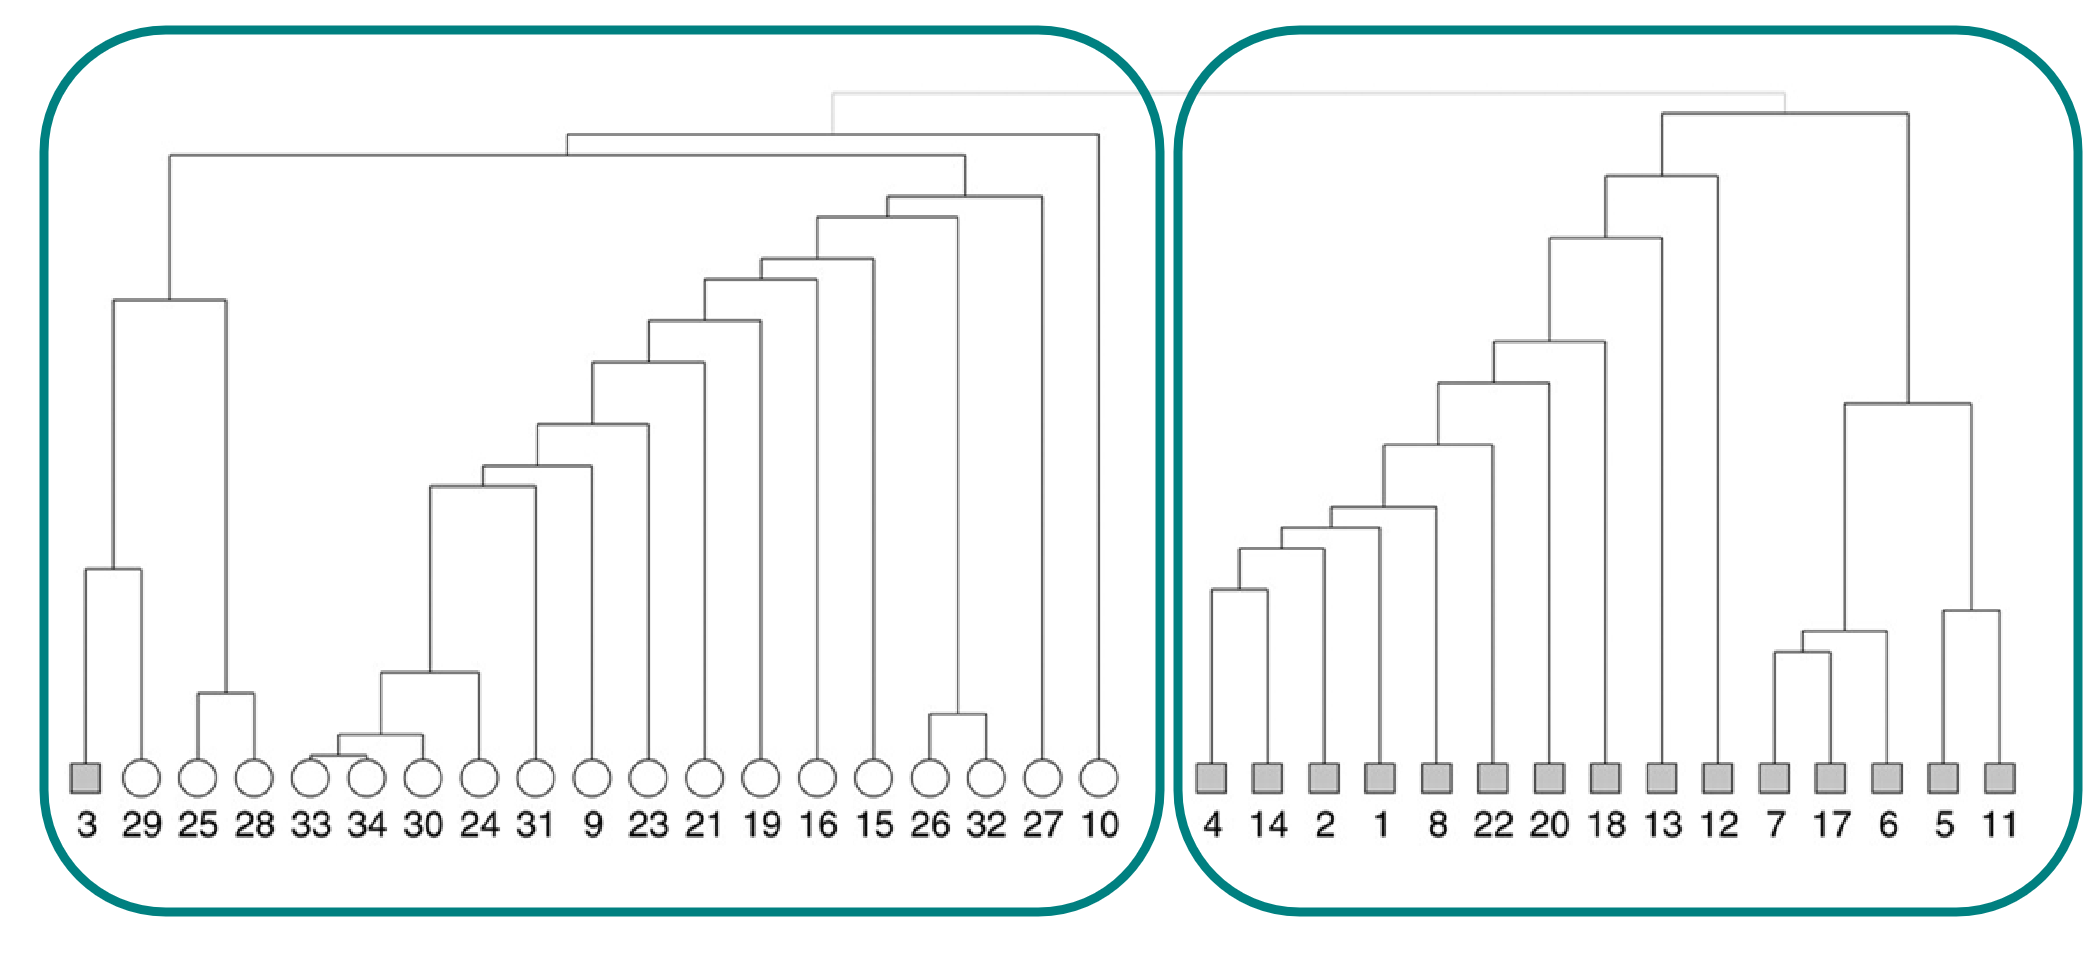
\includegraphics[width=\textwidth/2]{24.png}

dendrogram: tree diagram that shows the hierarchical relationship between objects



\section{Google's PageRank}
\subsection{PageRank: Intuition}
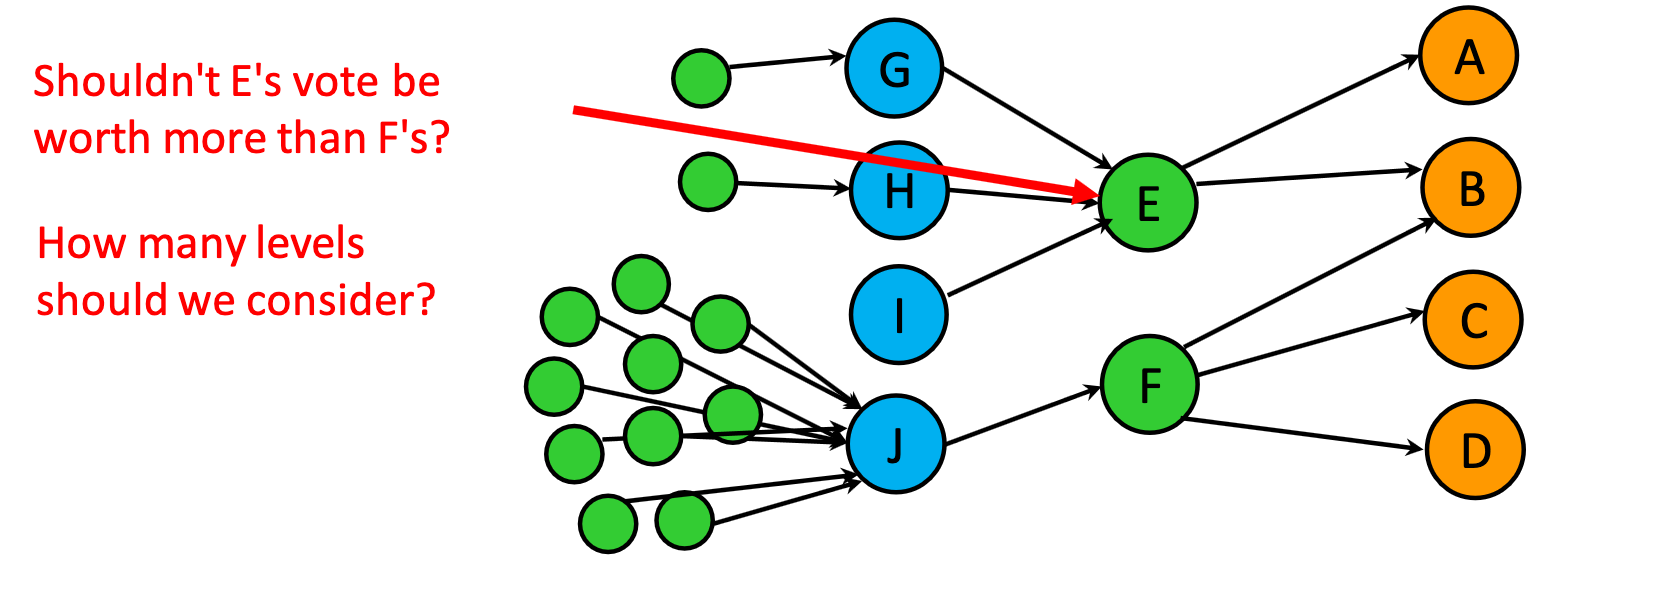
\includegraphics[width=\textwidth/2]{25.png}

Imagine a contest for The Web's Best Page

\begin{itemize}
    \item Initially, each page has one vote
    \item Each page votes for all the pages it has a link to
    \item To ensure fairness, pages voting for more than one page must split
    their vote equally between them
    \item Voting proceeds in rounds; in each round, each page has the number
    of votes it received in the previous round
    \item In practice, it's a little more complicated - but not much!
\end{itemize}

\subsection{PageRank}
Each page i is given a rank x$_i$

Goal: Assign the x$_i$ such that the rank of each page is
governed by the ranks of the pages linking to it:

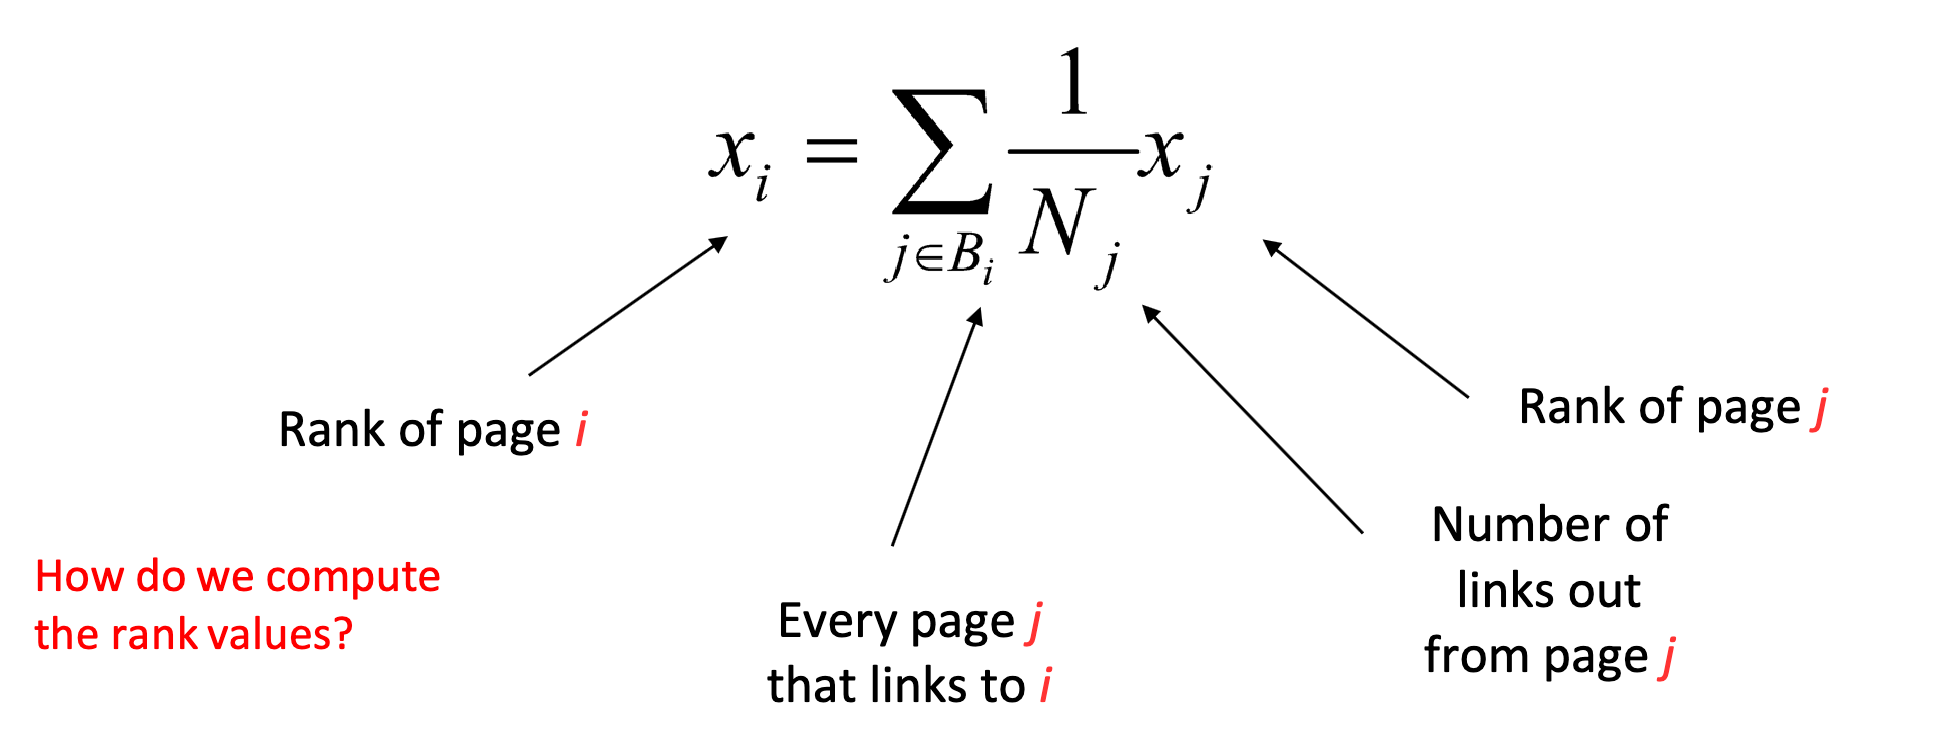
\includegraphics[width=\textwidth/2]{26.png}

\subsection{Iterative PageRank (simplified)}
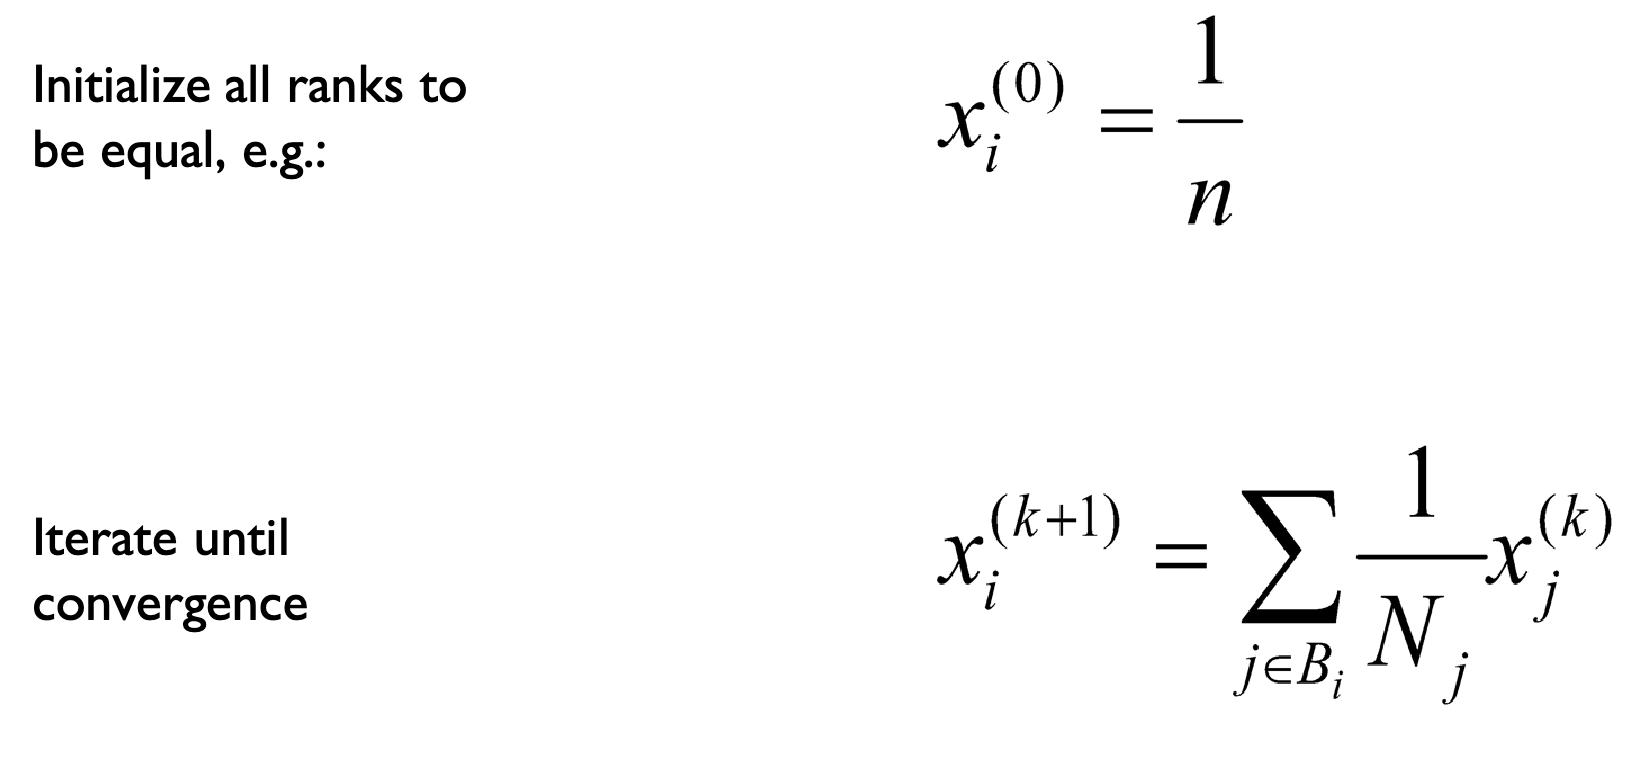
\includegraphics[width=\textwidth/2]{27.png}

\subsection{Example}
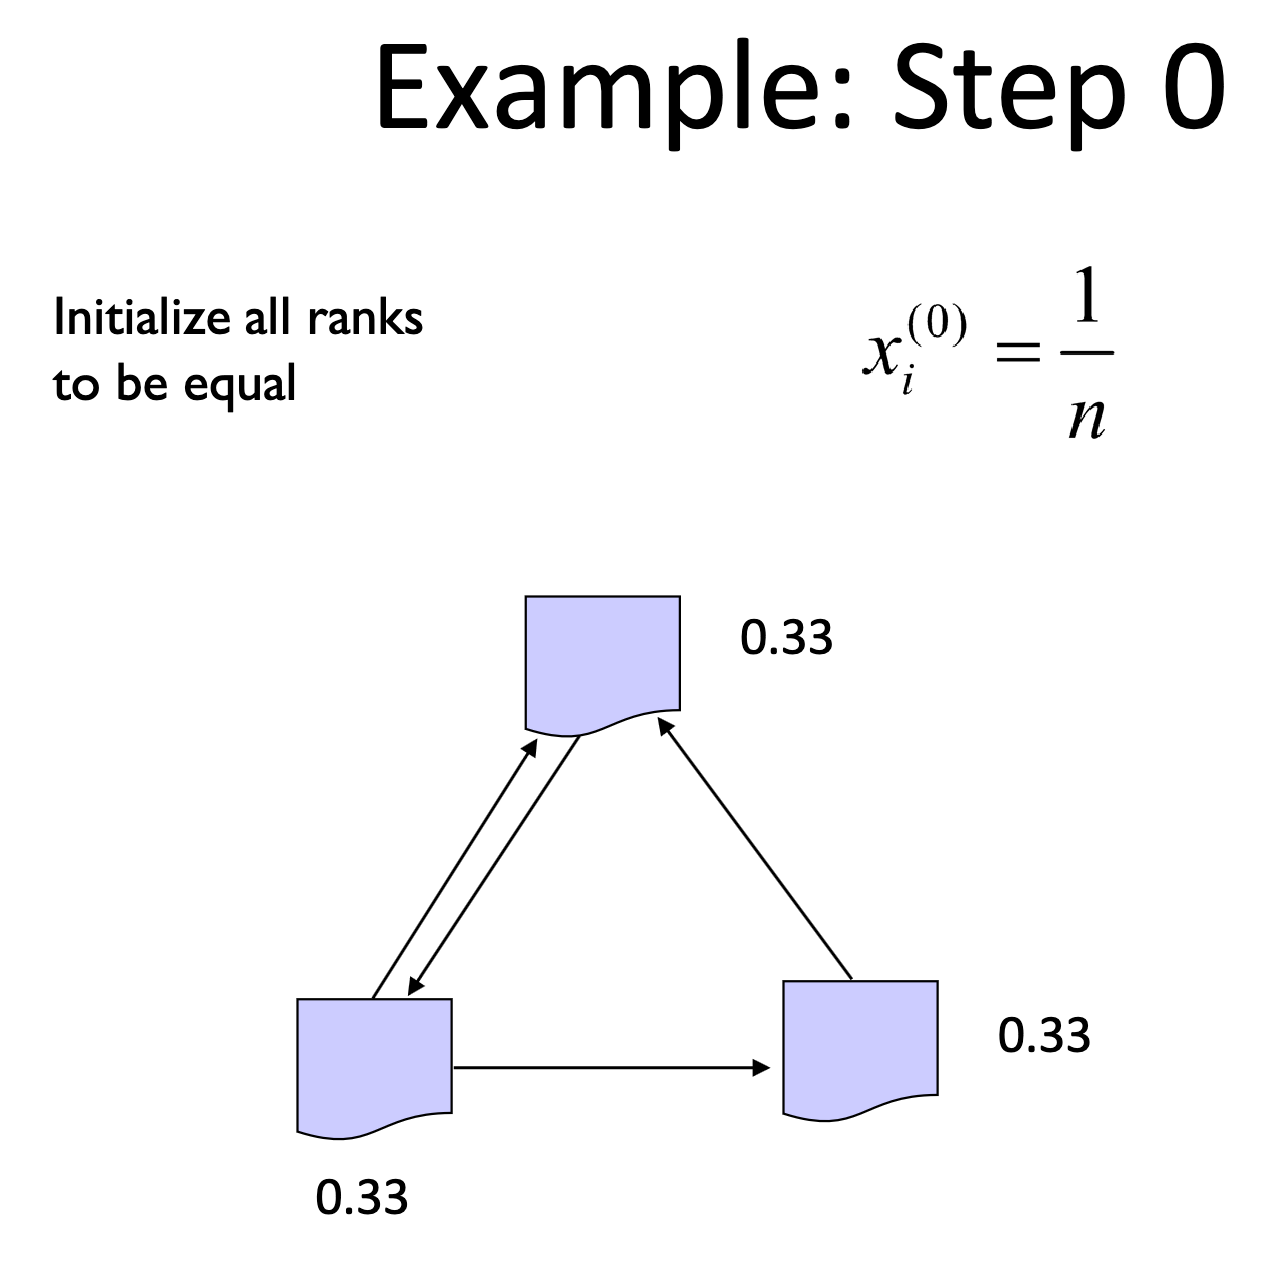
\includegraphics[width=\textwidth/3]{29.png}
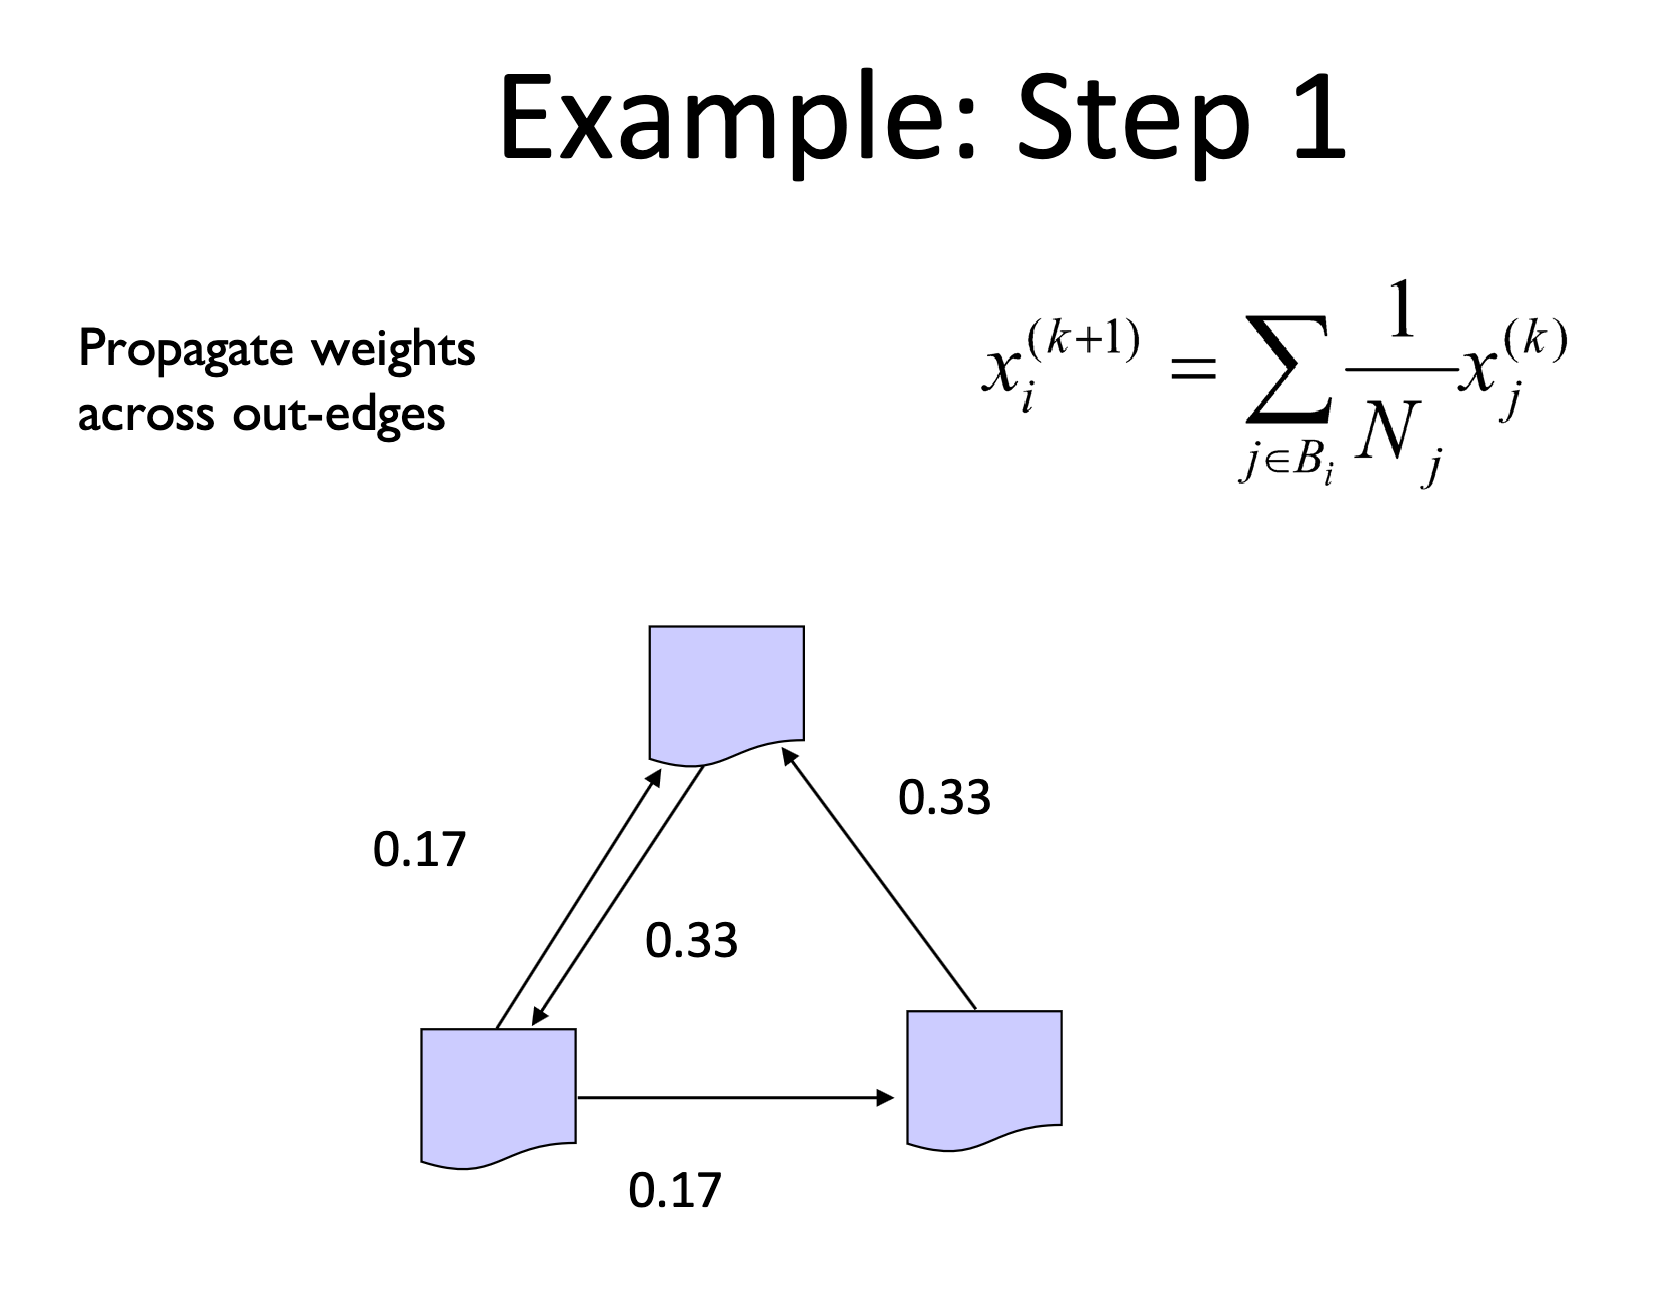
\includegraphics[width=\textwidth/2]{30.png}
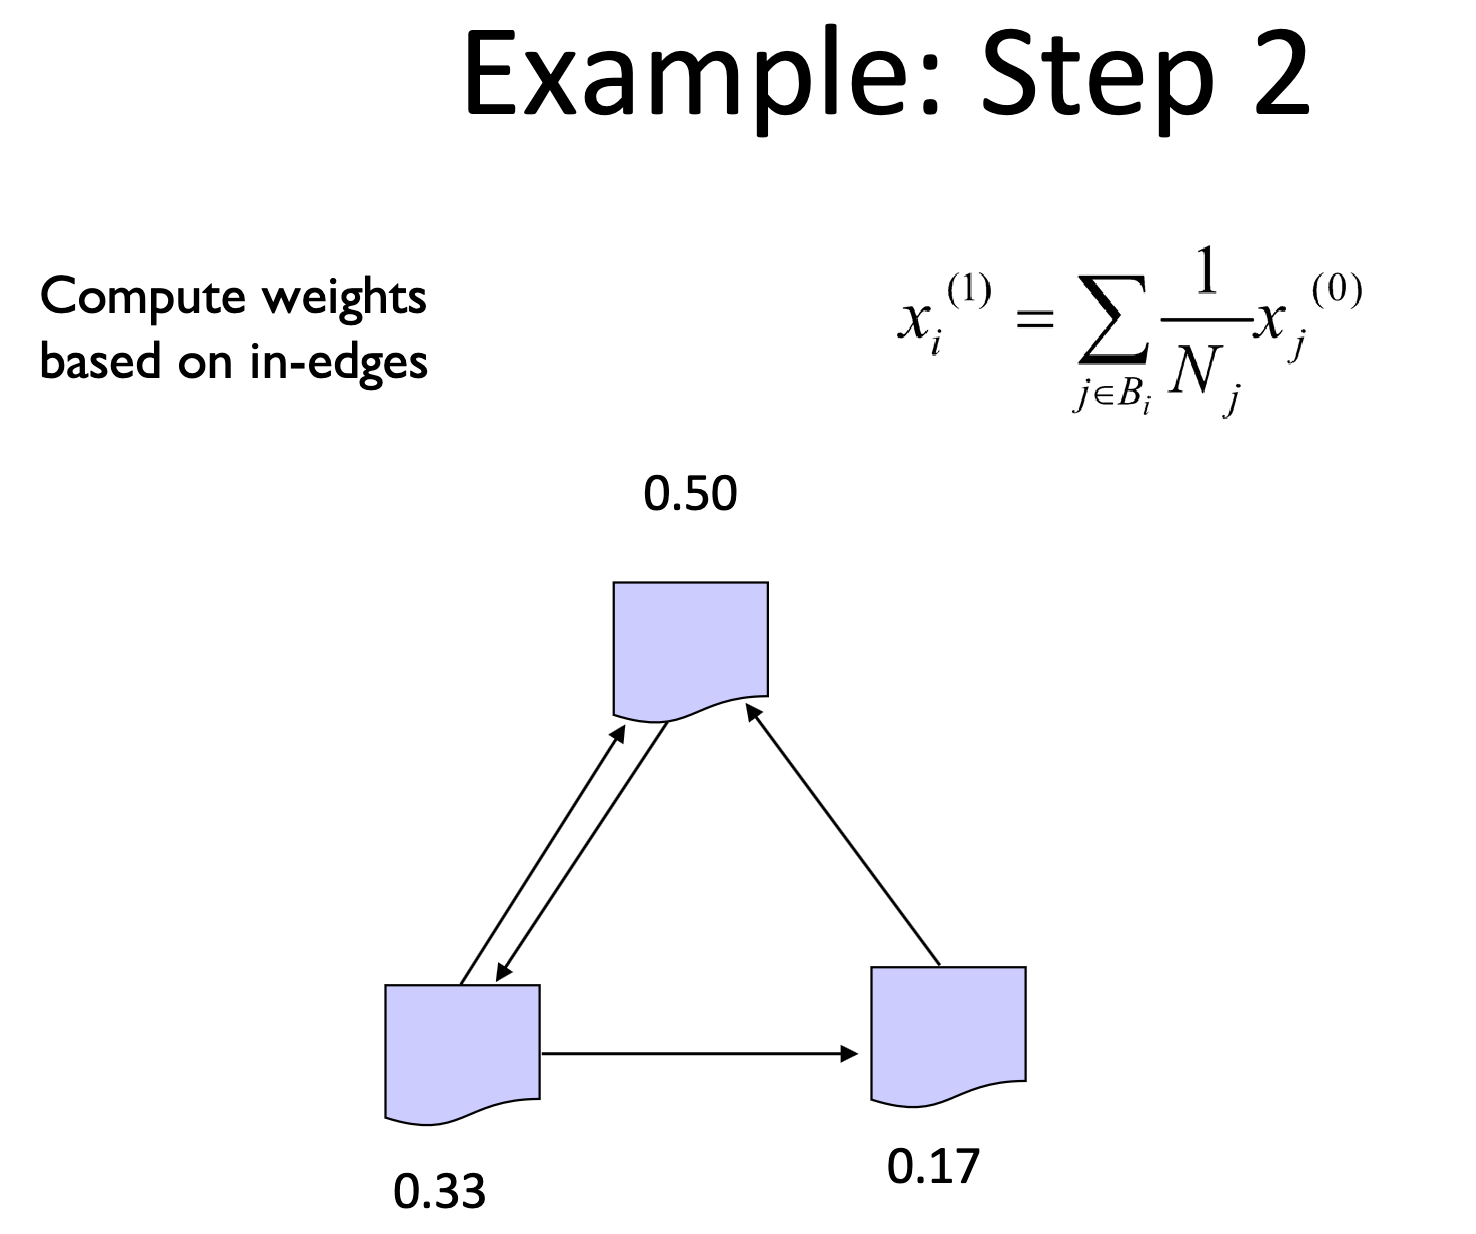
\includegraphics[width=\textwidth/2]{31.png}
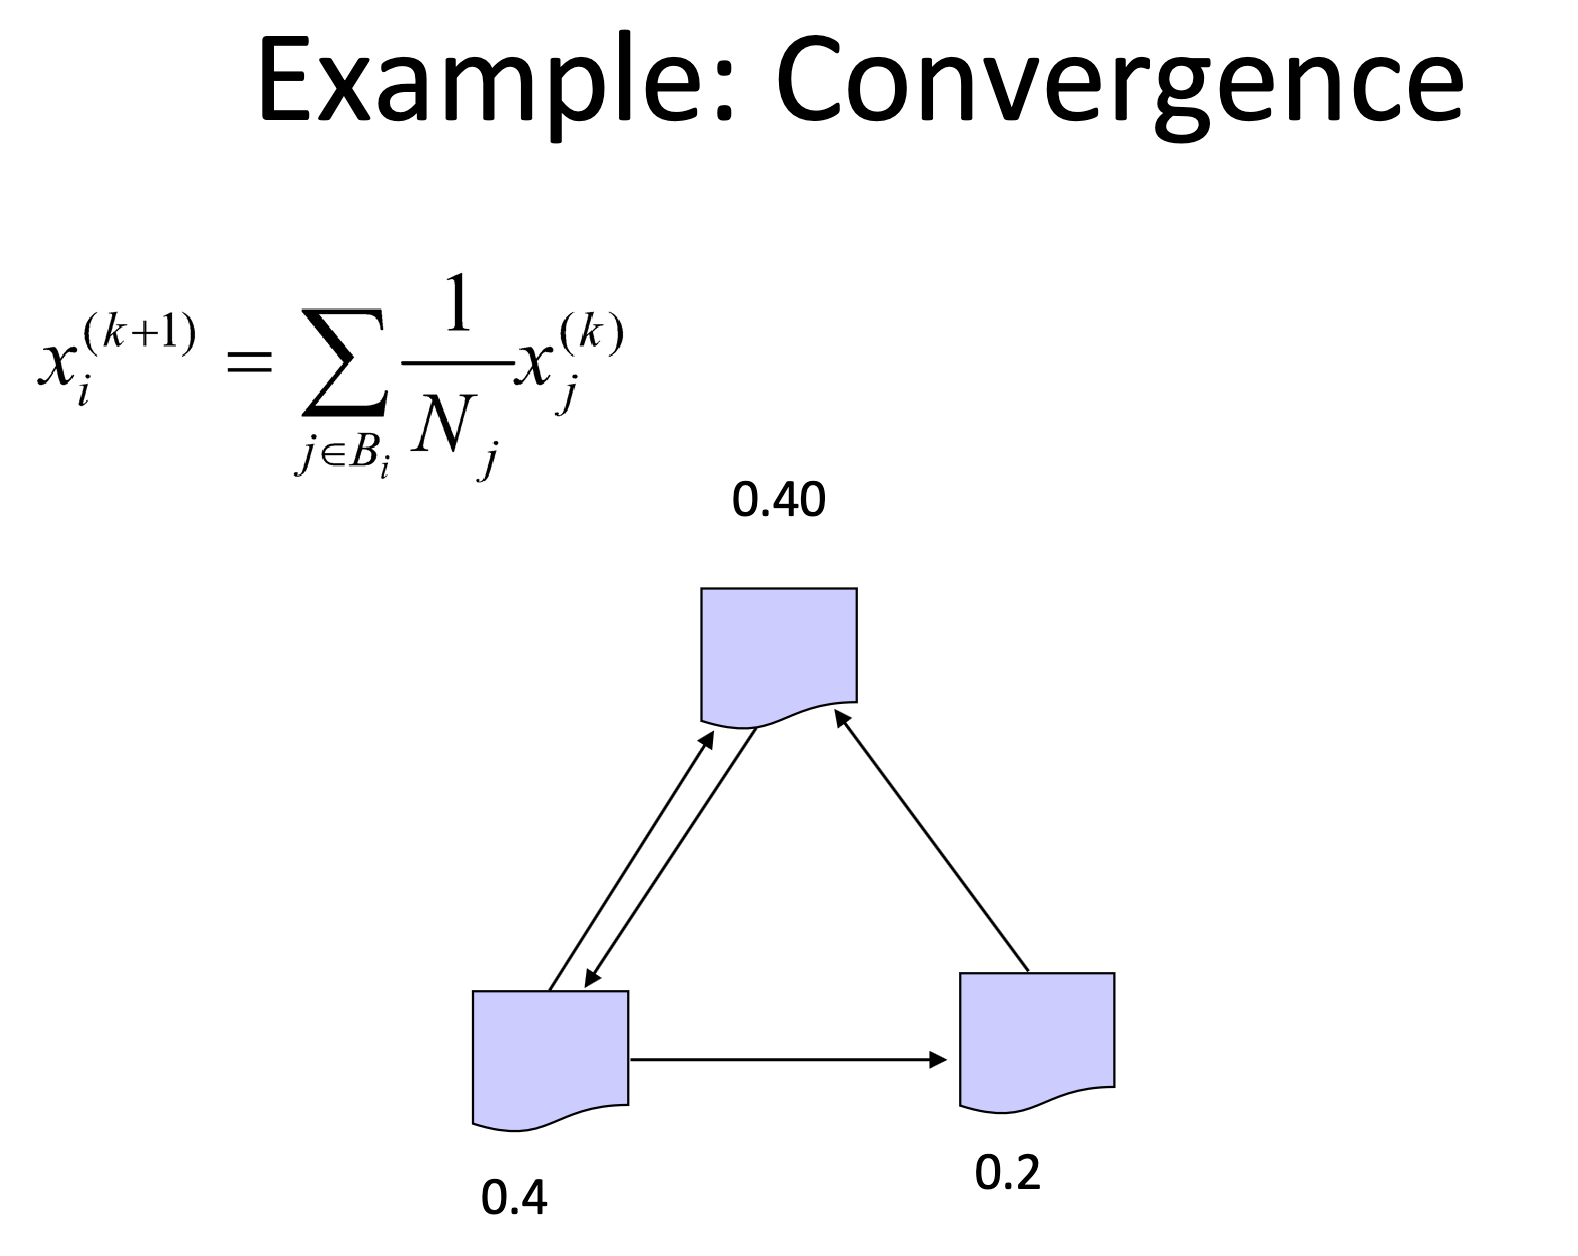
\includegraphics[width=\textwidth/2]{32.png}

\subsection{Naïve PageRank Algorithm Restated}
Let

\begin{itemize}
    \item N(p) = number outgoing links from page p
    \item B$_p$ = set of pages that back-link to page p
\end{itemize}


\includegraphics[width=\textwidth/4]{33.png}

Each page b distributes its importance to all of the pages it points to (so
we scale by 1/N(b))

Page p’s importance is increased by the importance of its back set

\subsection{In Linear Algebra formulation}
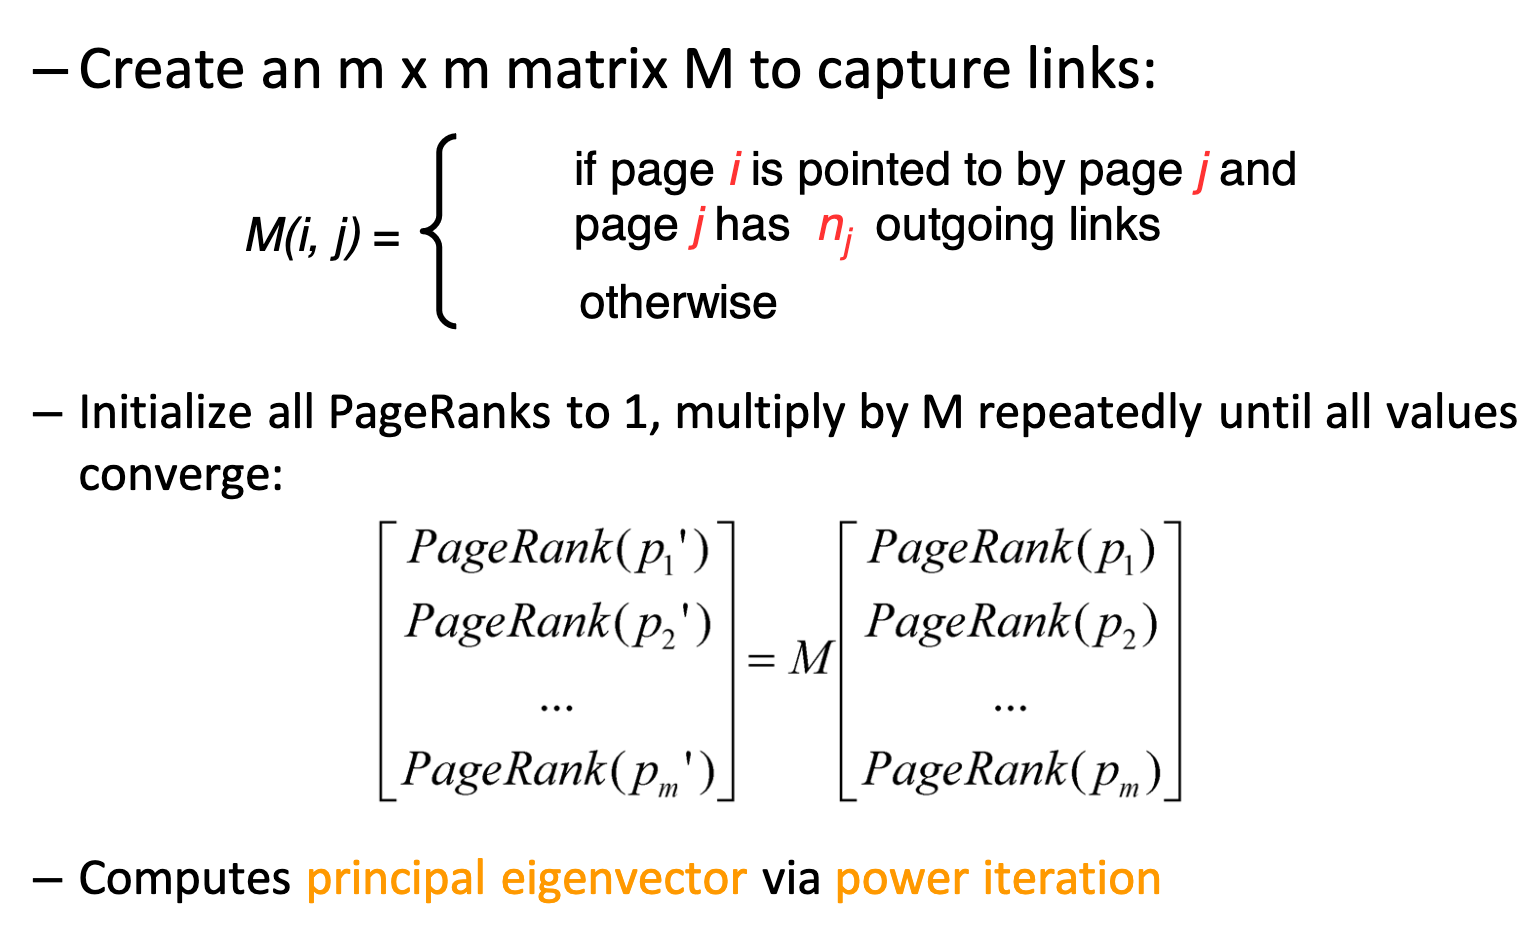
\includegraphics[width=\textwidth/2]{34.png}

\subsection{A Brief Example}
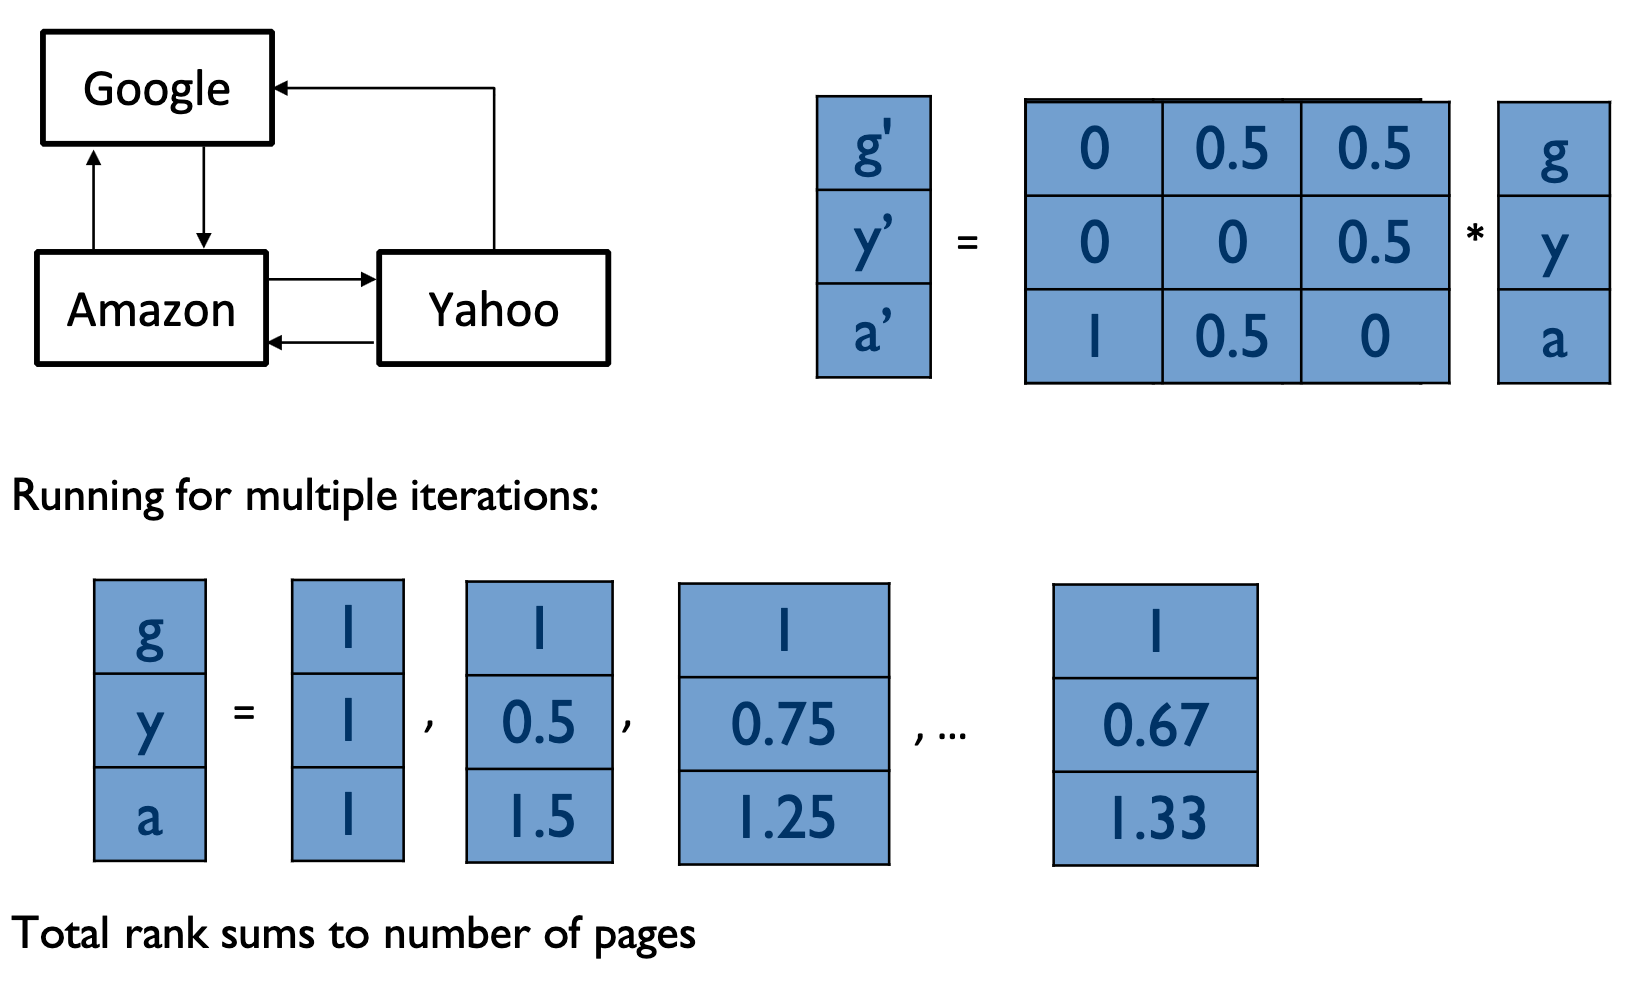
\includegraphics[width=\textwidth/2]{35.png}

\subsection{Random Surfer Model}
PageRank has an intuitive basis in random walks on graphs

Imagine a random surfer, who starts on a random page and, in each
step,

\begin{itemize}
    \item with probability d, clicks on a random link on the page
    \item with probability 1-d, jumps to a random page (bored?)
\end{itemize}

The PageRank of a page can be interpreted as the fraction of steps the
surfer spends on the corresponding page

Transition matrix can be interpreted as a Markov Chain

\subsection{Recap: PageRank}
Estimates absolute 'quality' or 'importance' of a given
page based on inbound links

\begin{itemize}
    \item Can be computed via fixpoint iteration
    \item Can be interpreted as the fraction of time a 'random
    surfer' would spend on the page
    \item Several refinements (not covered here)
\end{itemize}

An important factor for Google ranking of web pages, but
not the only one

Overall ranking is based on many factors (Google: >200)

Aside: What could be the other
200 factors?
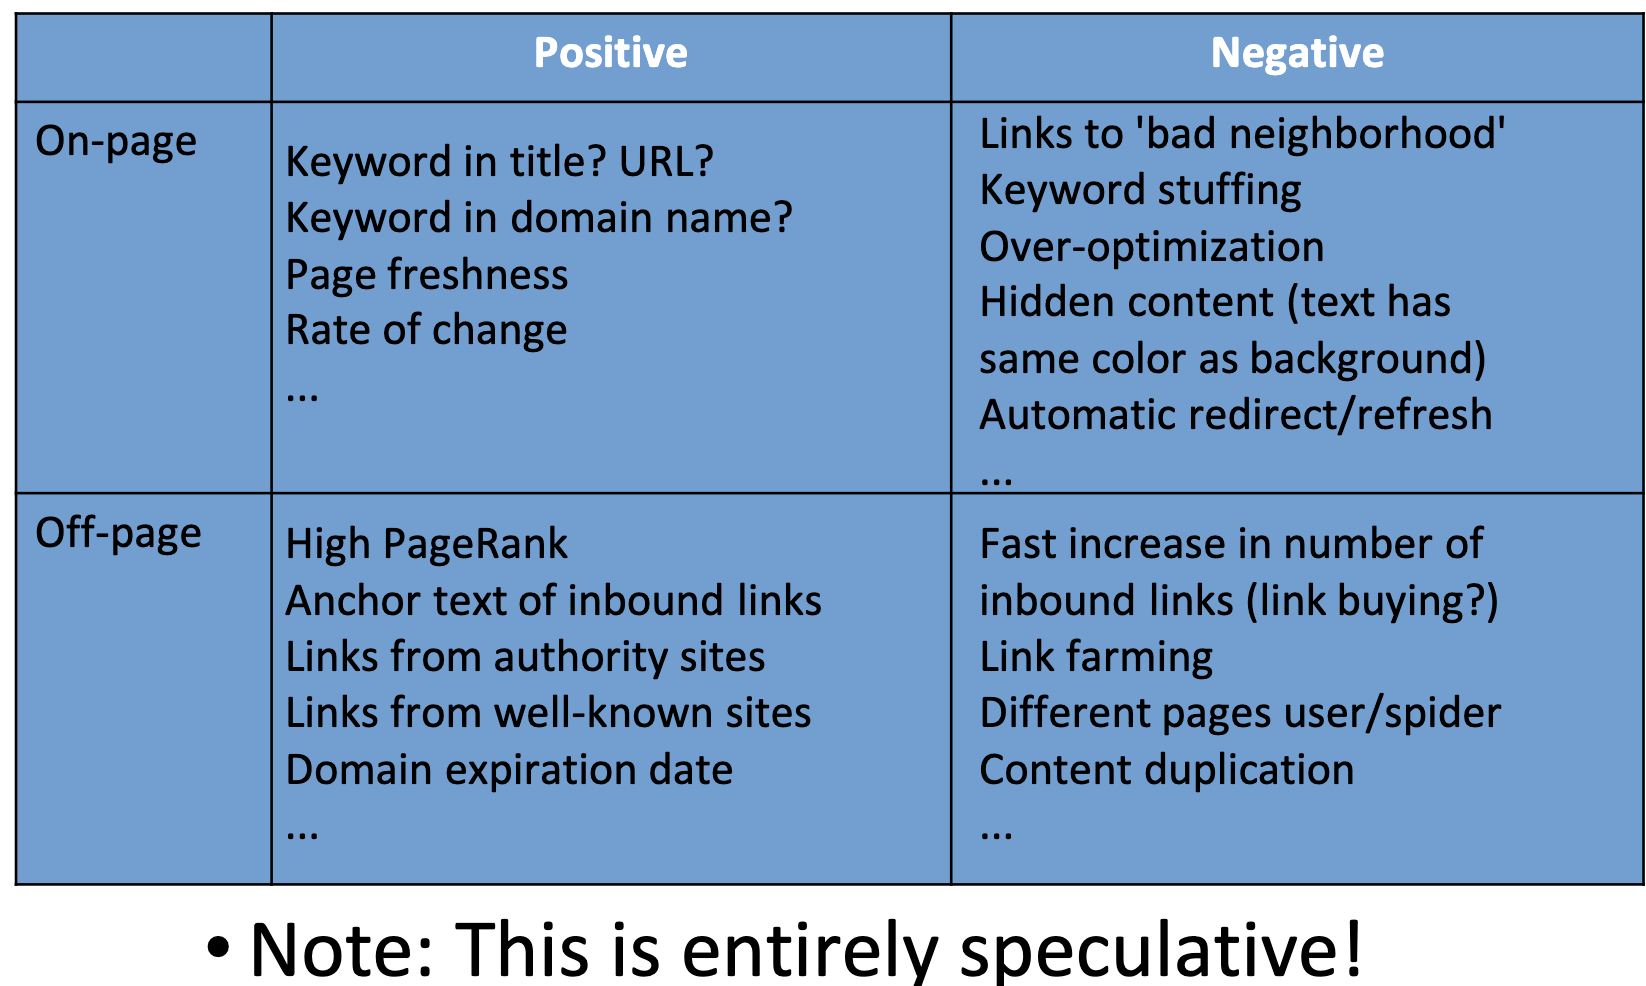
\includegraphics[width=\textwidth/2]{36.png}

\end{document}